\begin{abstract}
Poor health outcomes are shaped by more than medical conditions alone, yet there remains growing interest in understanding how social conditions, healthcare access, and insurance status influence health risk. This study examines demographic, socioeconomic, and healthcare access factors associated with poor self-rated health using the 2024 Behavioral Risk Factor Surveillance System (BRFSS), a national survey containing responses from more than 400,000 individuals. Drawing on variables related to insurance coverage, access barriers, chronic conditions, and socioeconomic status, this project evaluates factors that predict poor health outcomes and compares their relative importance through both statistical and machine learning approaches.

Exploratory analysis suggests that socioeconomic disadvantage and healthcare access barriers are strongly associated with poor health outcomes, in many cases more strongly than insurance status alone. Lower income and education levels, cost-related barriers to care, and chronic disease burden show especially strong relationships with poor health, while age also emerges as a major predictor. Although insurance coverage matters, initial findings suggest that broader structural conditions may carry greater predictive importance.

The analysis examines predictors of poor health using Logistic Regression, Random Forest, and XGBoost models, comparing their performance across multiple classification metrics and feature importance measures. Across models, factors such as physical health burden, chronic disease history, employment status, and education emerge as particularly influential predictors, while healthcare access barriers also contribute meaningfully to risk classification. More flexible machine learning models improve predictive performance and help capture nonlinear relationships that traditional approaches may overlook.

Overall, the findings suggest that poor health is driven by a combination of health burden, socioeconomic conditions, and barriers to care rather than insurance coverage alone. Future work should expand the analysis through additional health and geographic variables, refine predictive modeling approaches, and further investigate how these social and structural factors shape disparities in health outcomes.
\end{abstract}

\section{Introduction and Background}

\subsection{Introduction}

The relationship between the coverage of medical insurance and individual health outcomes has always been a core research topic in health policy. Theoretically, medical insurance can provide financial security for the insured population, thereby reducing the marginal cost of medical services, encouraging the popularization and utilization of medical services, and ultimately improving the health status of the group. However, in reality, the relationship between the coverage of medical insurance and individual health outcomes is very complex, and the final results are not as ideal as the theory suggests. There have been many randomized controlled experiments on this topic in history, such as the health insurance experiment of the RAND Corporation \cite{Manning1987Health} and the Oregon Health Insurance Experiment \cite{doi:10.1056/NEJMsa1212321}, whose results both indicate that although the coverage of medical insurance can increase the utilization rate of medical services and provide financial security for individuals, it cannot directly improve an individual's health.

Therefore, contemporary academic research has begun to focus on the differences in insurance types, such as comparing the differences in cost-effectiveness and the convenience of provided medical services between public medical programs and private insurance plans \cite{Allen_Gordon_Lee_Bhanja_Sommers_2021}. Apart from the differences in insurance types, there are also studies highlighting that even among those who have insurance, there are significant structural and behavioral barriers. Sommers et al. in their 2016 research emphasized the adverse effects of frequent interruptions in insurance continuity. Individuals frequently switch between different insurance types due to various objective factors, and may even lose their insurance completely, thus being forced to sever their long-term treatment relationships. Additionally, Benitez also pointed out in their research that whether healthcare providers are willing to accept patients usually depends on the reimbursement level, which also means that if the payment rate is too low, it will hinder patients from seeking treatment, even if these patients have insurance \cite{Benitez_Freed_Huang_Oladele_2024}.

In terms of methodology, this field has also undergone changes. For example, Clark et al. no longer solely rely on the traditional method of retrospective assessment of the average effect of policies, but increasingly adopt data-driven models to predict future risks \cite{Clark_Ommerborn_Moran_Brooks_Haas_Bates_Wright_2021}. In order to build a model that can identify and predict an individual's health status, this review synthesizes some relevant literature and conducts an analysis around four core themes. The first point is to analyze the causal relationship between medical insurance and an individual's health status, and then distinguish the differences among various types of insurance. Subsequently, it will further explore the structural barriers and behavioral mechanisms that hinder access to medical services, and finally evaluate the effectiveness of machine learning methods in the field of health prediction research.

\subsection{Background}

In the early days, research in the field of public health on health insurance was aimed at answering one question: Could reducing medical costs improve people's health levels? Manning and others conducted a very significant RAND Corporation health insurance experiment in order to obtain the answer \cite{Manning1987Health}. The results showed that although free insurance increased the rate of medical visits, the health levels of ordinary people did not significantly improve as a result. The overall rate of medical visits was still affected by multiple factors; for instance, the increase in cost-sharing would lead to a decrease in the number and frequency of medical services used by people. Although such measures were aimed at reducing unnecessary medical resource waste, they also reduced necessary preventive medical care, which was detrimental to personal health in the long run. However, a major limitation of this foundational study was its age; the data came from the 1970s, so it is difficult to directly apply these findings to the current complex healthcare system.

In 2013, the Oregon Health Insurance Experiment also confirmed this view. This study used a lottery system to assign Medicaid to some people while others did not receive it, thus conducting a comparative experiment. The results showed that Medicaid significantly increased medical utilization, including outpatient and preventive medical services, effectively reducing people's tendency towards depression, and providing economic security. However, from the data, physical clinical health indicators such as blood pressure and cholesterol did not show significant improvement in the short term \cite{doi:10.1056/NEJMsa1212321}. It is not ruled out that the experiment time was too short, which might not be long enough to capture long-term physiological health improvements. Additionally, Kronick analyzed national survey data in 2009. In this experiment, he more strictly controlled variables related to health status and socioeconomic factors to observe whether the mortality rate of the uninsured population significantly increased. After controlling for variables such as smoking and chronic diseases, the difference in mortality rates between insured and uninsured individuals did not have statistical significance. He pointed out that previous studies might have overestimated the impact of insurance on health levels \cite{Kronick_2009}.

These studies show that health insurance can significantly increase access to medical services, but it cannot guarantee that insured individuals directly achieve better health outcomes. After the Affordable Care Act was enacted, scholars no longer confined themselves to studying the simple opposition between "having insurance" and "not having insurance", but began to study the differences among various types of insurance, especially public medical plans and private insurance plans. Sommers et al. compared the situations in different states and found that the expansion patterns of public insurance and private insurance both reduced the number of uninsured individuals, but neither of the two models had a significant advantage in improving self-reported health assessment \cite{Sommers_Blendon_Orav_Epstein_2016}. However, there were significant differences in terms of cost and access to medical treatment between the two insurance models. Allen et al. compared the differences in total cost, out-of-pocket expenses,and price structure between the two insurance plans, and found that private insurance usually had more doctor resources, but patients' out-of-pocket expenses were almost ten times those of the Medicaid program. High costs are likely to prevent people from seeking medical services. On the other hand, although the Medicaid program is much cheaper for patients, due to the difficulty in scheduling regular outpatient visits, these patients often rely more on emergency rooms \cite{Allen_Gordon_Lee_Bhanja_Sommers_2021}.

Despite these problems, insurance type is still crucial for serious diseases. Albright et al. found that for women with gynecological cancer, having the Medicaid program was a key factor for early diagnosis and timely treatment \cite{Albright_Nasioudis_Craig_Moss_Latif_Ko_Haggerty_2021}. However, finding the right insurance plan does not ensure timely access to medical services, because regardless of the insurance type, systemic barriers exist objectively. Even if people have better insurance, structural barriers still prevent them from accessing medical services. A major issue is the unstable insurance coverage, and many people frequently switch between different insurances for various reasons. Sommers et al. found that nearly 25\% of low-income individuals lost or changed their insurance within a year. This led to their inability to continue seeing the same doctor or even to the interruption of their medical treatment altogether. Even when purchasing private insurance, the churn phenomenon did not significantly decrease \cite{Sommers_Gourevitch_Maylone_Blendon_Epstein_2016a}. Daw pointed out that for pregnant women, policy changes often cause them to frequently switch between Medicaid and private insurance plans, resulting in their inability to receive stable medical care \cite{Daw_Winkelman_Dalton_Kozhimannil_Admon_2020}.

This instability has actual consequences when it comes to patients with serious diseases: Rogers et al. showed that when patients with type 1 diabetes lose their insurance, their visit frequency increases sharply, and their blood sugar control also deteriorates \cite{Rogers_Lee_Tipirneni_Banerjee_Kim_2018}. In addition, Sudano and Baker also discovered a "lag effect", which refers to the fact that even if people regain their insurance, they will not immediately resume preventive examinations \cite{Sudano_Baker_2003}. It is clear that the instability of medical services has a significant negative impact on patients' health levels. Another obstacle comes from the providers of medical services. Benitez et al. found that insurance rates affect the services that medical service providers can provide. In states with a low reimbursement rate for Medicaid, the number of doctors treating Medicaid patients decreases accordingly. This creates a situation where people have insurance but cannot access medical services. Hoffman believes that when insured individuals use healthcare services more frequently, this is an "effective moral hazard", meaning that people will eventually receive the necessary treatment \cite{Hoffman2015Cost}.

\subsection{Methodologies in Literature}

Early research examining the relationship between health insurance coverage and health outcomes relied primarily on cross-sectional surveys and descriptive statistics to compare insured with uninsured populations \cite{Kronick_2009}. These studies documented disparities in access to care and utilization of preventive services, but were limited in their ability to establish causal relationships. As health policy research advanced, scholars increasingly adopted longitudinal, quasi-experimental, and experimental designs to improve causal inference and better isolate the effects of insurance coverage on health and well-being \cite{Sommers_Blendon_Orav_Epstein_2016}.

One of the key methodological approaches in this field is the use of randomized controlled trials. Baicker et al. (2013) employed a randomized lottery design in Oregon’s Medicaid expansion to estimate the causal effects of insurance coverage on health outcomes \cite{doi:10.1056/NEJMsa1212321}. Using lottery selection as a key variable for Medicaid enrollment, the authors addressed selection bias and common confounding factors in observational studies. Their analysis relied on linear probability models and clustered standard errors to account for household-level correlations. This experimental approach provides internal validity and serves as a benchmark for health policy research \cite{doi:10.1056/NEJMsa1212321} \cite{Manning1987Health}.

In addition to randomized designs, many studies have used quasi-experimental methods, particularly difference-in-differences (DiD) frameworks. Daw et al. (2020) and Albright et al. (2021) applied DiD models to evaluate Medicaid expansion across states with staggered adoption \cite{Albright_Nasioudis_Craig_Moss_Latif_Ko_Haggerty_2021}. These studies compared outcomes in expansion and non-expansion states before and after policy implementation, controlling for time-invariant differences and shared trends. Freund et al. (2019) used generalized estimating equations and piecewise time models to examine insurance stability following Massachusetts health reform \cite{Freund_LeClair_Terrin_Hanchate_Price_Moreno-Koehler_Suzukida_Kher_Byhoff_Kressin_2019}. These approaches allowed researchers to estimate the effects of policy changes on coverage continuity and access to care. Although DiD methods strengthen causal inference, they depend on the assumption that treatment and control groups follow similar trends before intervention \cite{Daw_Winkelman_Dalton_Kozhimannil_Admon_2020}.

Longitudinal survey designs have also played an important role in studying insurance instability. Sudano and Baker (2003) analyzed multiple waves of the Health and Retirement Study to assess how intermittent coverage affected preventive service use \cite{Sudano_Baker_2003}. Their weighted logistic regression models accounted for complex survey design and produced corrected relative risks. Sommers et al. (2016) similarly relied on longitudinal survey data to examine insurance “churning” following Affordable Care Act implementation \cite{Sommers_Blendon_Orav_Epstein_2016}. Longitudinal designs provide insight into how insurance status changes affect long-term outcomes, demonstrated through consistent links between coverage gaps, reduced service, and poorer health management \cite{Rogers_Lee_Tipirneni_Banerjee_Kim_2018}.

Several studies have relied on large administrative and survey datasets combined with multivariate regression techniques. Benitez et al. (2024) examined national survey data to examine how Medicaid reimbursement rates influenced access to care \cite{Benitez_Freed_Huang_Oladele_2024}. Their models incorporated both individual-level and state-level variables, allowing for multilevel analysis. Daw et al. (2020) used PRAMS data to study perinatal insurance transitions \cite{Daw_Winkelman_Dalton_Kozhimannil_Admon_2020}, while Freund et al. (2019) utilized electronic health and billing records to classify insurance status at each visit. These approaches show the value of combining clinical, demographic, and policy data when examining system performance \cite{Allen_Gordon_Lee_Bhanja_Sommers_2021}, \cite{Benitez_Freed_Huang_Oladele_2024}.

More recently, machine learning methods have been introduced to complement traditional statistical techniques. Clark et al. (2021) applied regularized logistic regression, random forests, and support vector machines to predict self-rated health using Behavioral Risk Factor Surveillance System data \cite{Clark_Ommerborn_Moran_Brooks_Haas_Bates_Wright_2021}. Their study used cross-validation and bootstrapping to improve model stability and addressed missing data through multiple imputation. Model performance was evaluated using area under the curve statistics, and feature importance measures identified key predictors. Although these methods are not designed for causal inference, they provide additional insights into complex relationships among behavioral and access-related factors \cite{Clark_Ommerborn_Moran_Brooks_Haas_Bates_Wright_2021},\cite{BRFSS2024}.

Across the literature, most studies rely on observational or quasi-experimental data, which introduces potential bias from unobserved confounding, measurement error, and self-reporting \cite{Kronick_2009}. Many analyses depend on self-reported insurance status and health behaviors, which may be affected by recall bias, while quasi-experimental designs may be influenced by policy endogeneity and regional differences \cite{Sommers2017InsuranceHealth}. Although randomized studies such as the Oregon experiment reduce many of these concerns, they remain rare due to ethical and practical constraints \cite{doi:10.1056/NEJMsa1212321}. Survey-based studies, including Sommers et al. (2016), also face limitations in establishing causality despite extensive adjustment \cite{Sommers_Blendon_Orav_Epstein_2016}. Outcome measurement presents an additional challenge, as studies vary between clinical indicators and subjective assessments, limiting cross-study comparability \cite{Clark_Ommerborn_Moran_Brooks_Haas_Bates_Wright_2021}. Furthermore, many datasets lack detailed information on neighborhood context, provider availability, and social support, restricting analyses of structural drivers of health disparities \cite{XIE20251412}, \cite{Benitez_Freed_Huang_Oladele_2024}

\subsection{Overall Project Plan}

Our project aims to identify the major non-clinical factors associated with poor health and evaluate how well these factors can be used to predict high-risk individuals. Using the 2024 BRFSS LLCP dataset, we focus on health insurance status, healthcare access barriers, socioeconomic conditions, demographic characteristics, and selected health history variables. The project follows a complete data science workflow: selecting relevant BRFSS variables, cleaning nonresponse codes, handling missing values, creating a binary poor-health outcome, and preparing the data for predictive modeling. Our analysis plans to compare Logistic Regression, Random Forest, and XGBoost using multiple metrics. Because the goal is early identification of high-risk individuals, certain model performance metrics such as recall and F1 score are especially important. Overall, the project examines whether insurance alone predicts poor health, or whether broader socioeconomic and access-related factors provide stronger predictive information.

\section{Methods}

\subsection{Data Source and Variable Selection}

This project uses the 2024 Behavioral Risk Factor Surveillance System (BRFSS) dataset from the Centers for Disease Control and Prevention (CDC). The BRFSS is one of the largest annual health survey systems in the world. It collects information on health-related risk behaviors, chronic conditions, healthcare use, and preventive services among U.S. adults. The 2024 BRFSS dataset includes responses from over 400,000 American adults and contains more than 300 variables. Based on the goal of this project, which is to identify people at high risk of reporting poor health using non-clinical factors, we did not use clinical disease diagnosis variables as our main predictors. Instead, we selected approximately 14 non-clinical variables from the original dataset related to insurance coverage, healthcare access, socioeconomic status, and demographic background for exploratory analysis and machine learning modeling.

The outcome variable in this project is \texttt{GENHLTH}, which represents each respondent's self-reported general health status. The predictor variables are organized into four groups. Insurance-related variables include health insurance status \texttt{\_HLTHPL2} and primary insurance type \texttt{PRIMINS2}. Healthcare access variables include whether the respondent has a personal doctor \texttt{PERSDOC3}, whether they were unable to see a doctor due to cost \texttt{MEDCOST1}, and when they last had a routine checkup \texttt{CHECKUP1}. Socioeconomic variables include income level \texttt{\_INCOMG1}, education level \texttt{\_EDUCAG}, employment status \texttt{EMPLOY1}, and homeownership status \texttt{RENTHOM1}. Demographic variables include age group \texttt{\_AGE\_G}, sex \texttt{SEXVAR}, race/ethnicity group \texttt{\_RACEGR3}, and urban/rural status \texttt{\_METSTAT}.

After an initial exploration of the dataset, we found that the proportion of respondents reporting poor health was noticeably lower than those who did not, with the two groups at roughly a 1:4 ratio. To better align the model with the project's goal of identifying high-risk individuals, we recoded \texttt{GENHLTH} into a binary outcome variable called \texttt{poor\_health}. Respondents who reported fair or poor general health were coded as 1, while those with all other valid health ratings were coded as 0. Once this outcome variable was created, the original \texttt{GENHLTH} variable was excluded from the predictors to avoid data leakage.

\subsection{Data Cleaning and Feature Engineering}
After selecting the variables needed for this project, we first examined the value distribution of each variable. Because the original data come from a survey, some respondents refused to answer certain questions or indicated that they did not know the answer. Some of these responses are considered invalid, while others carry special meanings. Many variables in the BRFSS use numeric codes to represent these non-response options. For most variables, these codes cannot be treated as meaningful categories, so we recoded them as missing values before creating the final analytic dataset.

For the outcome variable \texttt{GENHLTH}, only values 1 through 5 were kept as valid health ratings, while 7 and 9 were treated as missing. For the main predictor variables, we also handled invalid and non-response values accordingly. For example, invalid responses in the healthcare access variables \texttt{PERSDOC3}, \texttt{MEDCOST1}, and \texttt{CHECKUP1}, the socioeconomic variables \texttt{\_EDUCAG}, \texttt{EMPLOY1}, and \texttt{RENTHOM1}, and the demographic variable \texttt{\_RACEGR3} were all recoded as missing. Afterward, for core variables with a low proportion of missing values, we removed rows containing missing values to obtain a cleaner analytic sample. For variables where an ``Unknown'' response might still carry useful information, such as income level and insurance type, we did not drop those rows. Instead, we retained these values as an ``Unknown'' category.

To make the subsequent analysis easier to follow, we also renamed the variables. For example, \texttt{\_HLTHPL2} was renamed \texttt{has\_insurance}, \texttt{PERSDOC3} was renamed \texttt{has\_personal\_doctor}, \texttt{MEDCOST1} was renamed \texttt{cost\_barrier}, \texttt{CHECKUP1} was renamed \texttt{last\_checkup\_time}, \texttt{\_INCOMG1} was renamed \texttt{income\_level}, and \texttt{\_EDUCAG} was renamed \texttt{education\_level}. Some binary variables were also recoded for modeling purposes. For example, in \texttt{has\_insurance}, respondents with insurance were coded as 1 and those without insurance were coded as 0. In \texttt{cost\_barrier}, respondents who were unable to see a doctor due to cost were coded as 1, while respondents without this barrier were coded as 0. Sex was recoded into \texttt{is\_female}, and urban/rural status was recoded into \texttt{is\_urban}.

The original \texttt{GENHLTH} variable was recoded into a binary outcome variable called \texttt{poor\_health}. Respondents who reported fair or poor general health were coded as 1, and those who reported excellent, very good, or good health were coded as 0. We used this binary variable because the goal of this project is to identify respondents at higher risk of reporting poor health. After creating \texttt{poor\_health}, the original \texttt{GENHLTH} variable was excluded from the predictors to avoid data leakage.

Categorical variables were also converted into more interpretable labels to support later analysis and visualization. For example, income level was labeled with categories ranging from \texttt{<15k} to \texttt{200k+}, education level was divided into four tiers, and employment status was named according to the original BRFSS response categories. Primary insurance type was first converted into detailed labels and then grouped into broader categories, including private insurance, public insurance, military or VA coverage, other public or tribal coverage, no coverage, and unknown. This grouped insurance variable was used in the layered models because it retains more information about insurance type than a simple insured/uninsured variable while still including the no-coverage group.

\subsection{Exploratory Data Analysis}
Before building any machine learning models, we performed exploratory data analysis (EDA) to understand the basic structure of the dataset and the relationships between the selected non-clinical variables and the binary outcome variable. We started by examining the distribution of \texttt{poor\_health} by comparing the number of respondents who reported poor health with those who did not. We did this because a large imbalance between the two classes can affect how the models are trained and evaluated.

We then used our research questions and the findings from the literature review to guide the first set of visualizations. Since insurance coverage and healthcare access were important to the project, we first used bar charts to explore how poor-health rates differed across insurance-related variables, including insurance status and grouped insurance type. The purpose of this step was to check whether insurance information showed clear differences in poor-health rates. In addition, we used bar charts and grouped summary tables to compare poor-health rates across the main predictor groups, including healthcare access, socioeconomic status, and demographic variables. For categorical variables, we compared the proportion of respondents reporting poor health within each category rather than only comparing raw counts. This approach allowed for a fairer comparison across groups of different sizes. For example, we examined poor-health rates across variables such as insurance type, cost barrier, income level, education level, employment status, homeownership status, age group, race/ethnicity group, and urban/rural status.

Beyond exploring individual variables, we also created two grouped bar charts using \texttt{cost\_barrier} as the grouping variable. We chose \texttt{cost\_barrier} because it directly indicates whether a respondent was unable to see a doctor due to cost, which is closely related to our research question about access-to-care barriers. It also showed a clear difference in poor-health rates during the initial EDA, making it useful for further group comparisons. Specifically, we compared poor-health rates across different income levels and cost barrier statuses, and also across different insurance statuses and cost barrier statuses. These two comparisons connect healthcare affordability, socioeconomic status, and insurance coverage. The goal was to describe patterns of cost-related healthcare barriers across different groups rather than to draw causal conclusions.

Finally, we created two summary visualizations to compare the selected predictor variables overall. The first chart calculated the descriptive separation for each variable, defined as the difference between the highest and lowest poor-health rates across that variable's categories. The purpose of this chart was to see which variables showed a clearer difference in poor-health rates during the EDA. The second chart used Cramér's V to create a categorical association heatmap. Because most of the predictor variables in this project are categorical, Cramér's V helped us check the strength of association between variables and check for possible overlap among them before building models. These EDA results were used to guide model design and interpretation, but they were not treated as causal evidence.

\subsection{Layered Model Design}
In this project, we used a layered model design to compare how different groups of non-clinical variables performed in the models. Rather than putting all variables into the model at once, we added them step by step based on our earlier variable groups. The goal was to observe whether each new group of variables improved model performance beyond the previous model.

Model 1 included only insurance information, using \texttt{insurance\_type\_grouped}. We used the grouped insurance type variable because it keeps information about different insurance types while also including the no-coverage group. Model 2 added healthcare access variables, including \texttt{cost\_barrier}, \texttt{has\_personal\_doctor}, and \texttt{last\_checkup\_time}. Model 3 further added socioeconomic variables, including \texttt{income\_level}, \texttt{education\_level}, \texttt{employment\_status}, and \texttt{home\_ownership}. Model 4 was the full non-clinical model and added demographic variables, including \texttt{age\_group}, \texttt{is\_female}, \texttt{race\_group}, and \texttt{is\_urban}.

This layered design was based on our research questions. It allowed us to compare model performance using insurance information alone and then check whether performance changed after adding healthcare access, socioeconomic status, and demographic background in order. By comparing all four models, we could assess whether healthcare access and socioeconomic variables provided additional predictive information beyond insurance information alone.

\subsection{Machine Learning Methods}
We used three supervised classification models to predict the binary outcome variable \texttt{poor\_health}: Logistic Regression, Random Forest, and XGBoost. Logistic Regression was used as the baseline model because it can estimate the probability of poor health and allows us to examine the direction of the relationship between each predictor and the outcome through its coefficients. Random Forest was chosen because it can capture non-linear patterns and possible interactions between variables without requiring us to specify those interactions manually. XGBoost was included because it is a boosted tree model that often works well with structured tabular data and can improve prediction by building multiple trees in sequence. By comparing these three models, we can assess whether a simpler model is enough for this task or whether tree-based models provide stronger predictive performance.

We divided the predictor variables into two groups: categorical variables and binary variables. Categorical variables were handled using one-hot encoding, while binary variables were kept in numeric form. We did not apply feature scaling during model preparation. Although scaling is often recommended for Logistic Regression, it was not necessary here because the variables included in the model were either binary or one-hot encoded categorical variables, with no continuous variables included. For Random Forest and XGBoost, scaling is not required because tree-based models are not sensitive to the scale of variables.

To make the code more efficient and keep the modeling steps consistent, we built machine learning pipelines to handle preprocessing and model training together. This ensured that the same preprocessing steps were applied during both training and testing, and it also reduced the risk of data leakage. The dataset was split into a training set and a testing set, and the models were trained only on the training data before being evaluated on the testing data.

Because \texttt{poor\_health} was imbalanced and made up a smaller share of the dataset, relying on accuracy alone could be misleading. Logistic Regression and Random Forest were both configured with balanced class weights, while XGBoost used a positive-class weight calculated from the ratio between the majority class and the minority class. This allowed each model to pay more attention to the smaller poor-health group during training.

\subsection{Model Evaluation}
In this project, we evaluated model performance from several angles, using both cross-validation results during training and final performance on the test set. The cleaned dataset was first split into a training set and a testing set using an 80/20 split. The training set was used to train the models and compare the layered model designs, while the testing set was held out until the end for final evaluation.

During the training phase, we used 3-fold stratified cross-validation to compare the four layered models. Stratification was used to keep the ratio of poor-health to non-poor-health respondents similar in each fold. This was important because \texttt{poor\_health} had a class imbalance. Compared with using only one train/test split, cross-validation gave us a more stable way to compare models. Based on model performance across different metrics during training, we selected Model 4, which included all variable groups, as the final model structure for test-set comparison.

For evaluation metrics, we used accuracy, precision, recall, F1 score, and ROC-AUC. Accuracy measures the overall proportion of correct predictions, but it can be misleading when one class is much larger than the other. For this reason, accuracy was not used as the only measure of model performance. Since the main goal of this project was to identify respondents in the poor-health group, recall was especially important. Recall measures how many true poor-health cases the model correctly identified. Precision measures how many respondents predicted as poor health were actually in the poor-health group. F1 score balances precision and recall, while ROC-AUC measures the model's ability to separate the two classes across different thresholds.

After completing the cross-validation comparisons, we evaluated the final models on the test set and created confusion matrices and ROC curves. The confusion matrices were used to examine how each model classified respondents into the poor-health and non-poor-health groups at a specific threshold. This was useful because we wanted to see whether the models missed many true poor-health cases. The ROC curves were used to compare how well the three models ranked respondents by their predicted risk of reporting poor health across different thresholds.

In addition to reporting evaluation metrics in tables, we created several visualizations to compare model performance. Line plots were used to show how ROC-AUC and F1 score changed across the four layered models. This helped us see whether adding new predictor groups improved performance. For the final full models, we used grouped bar charts to compare accuracy, precision, recall, F1 score, and ROC-AUC on the test set. We also used ROC curves and precision-recall curves to compare how well the final models ranked respondents by predicted poor-health risk. Finally, coefficient and feature importance plots were used to support model interpretation after performance was evaluated.

\section{Results}

\subsection{Exploratory Data Analysis Results}

We first examined the distribution of the binary outcome variable, \texttt{poor\_health}. As shown in Figure~\ref{fig:poor_health_distribution}, the final analytic sample included 322,568 respondents in the non-poor-health group and 77,197 respondents in the poor-health group. This means that 80.7\% of respondents were classified as not reporting poor health, while 19.3\% were classified as reporting poor health.

\begin{figure}[H]
    \centering
    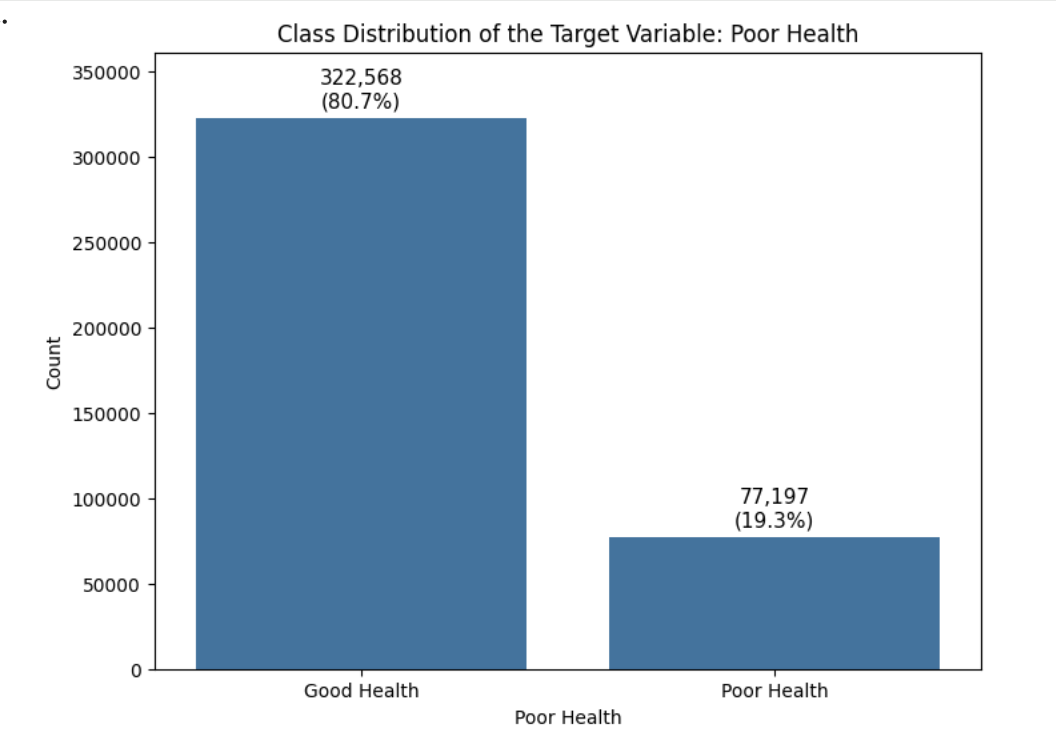
\includegraphics[width=0.75\textwidth]{image/poor_health_distribution.png}
    \caption{Class distribution of the binary poor health outcome.}
    \label{fig:poor_health_distribution}
\end{figure}

\begin{table}[H]
\centering
\caption{Distribution of the Binary Poor Health Outcome}
\label{tab:poor_health_distribution}
\begin{tabular}{lrr}
\toprule
Outcome Group & Count & Percentage \\
\midrule
Not poor health & 322,568 & 80.7\% \\
Poor health & 77,197 & 19.3\% \\
\bottomrule
\end{tabular}
\end{table}

The distribution shows a clear class imbalance in the outcome variable. The poor-health group was much smaller than the non-poor-health group, with roughly one poor-health respondent for every four non-poor-health respondents. This was important for model evaluation because a model could achieve a high accuracy score by mostly predicting the larger group. Because of this, later model evaluation also focused on recall, F1 score, and ROC-AUC rather than accuracy alone.

\begin{figure}[H]
    \centering
    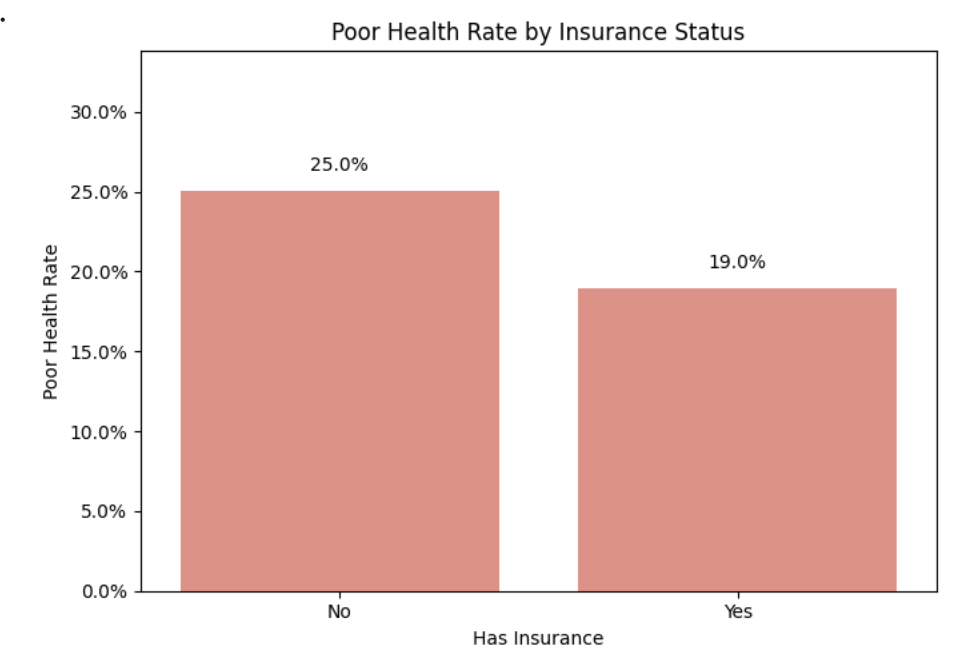
\includegraphics[width=0.75\textwidth]{image/poor_health_by_insurance_status.png}
    \caption{Poor-health rate by insurance status.}
    \label{fig:poor_health_insurance_status}
\end{figure}
Figure~\ref{fig:poor_health_insurance_status} compares the poor-health rate between respondents with and without health insurance. Respondents without insurance had a poor-health rate of 25.0\%, while respondents with insurance had a lower rate of 19.0\%. This shows that the uninsured group had a higher share of respondents reporting fair or poor general health. However, the difference is not large enough to explain poor health by insurance status alone, so we also examined more detailed insurance type and healthcare access variables in the next steps.

\begin{figure}[H]
    \centering
    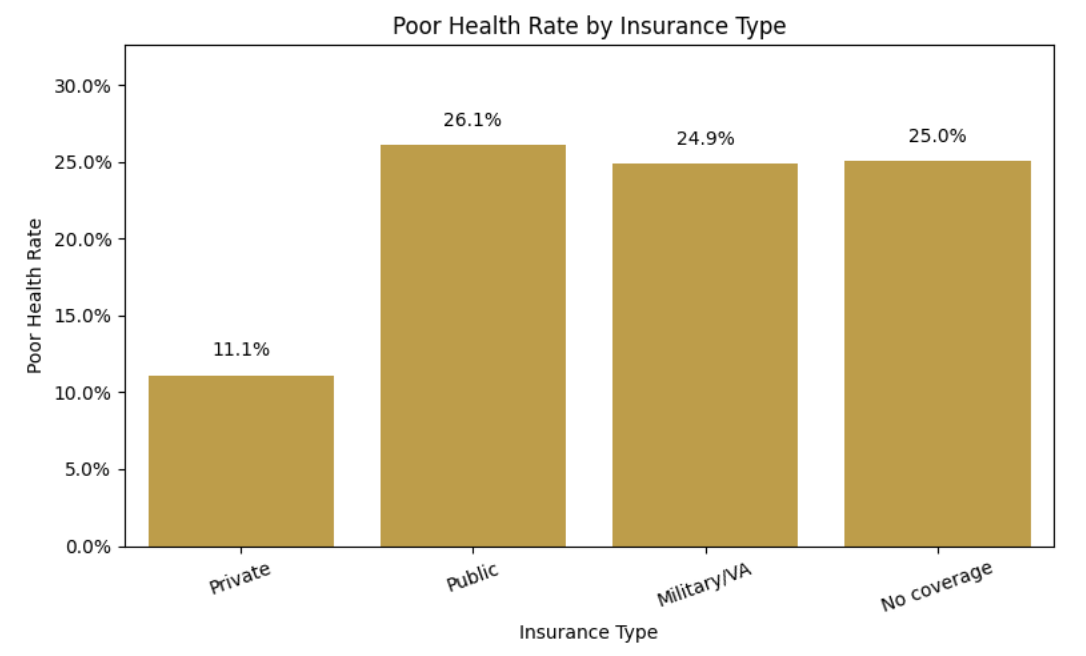
\includegraphics[width=0.75\textwidth]{image/poor_health_by_insurance_type.png}
    \caption{Poor-health rate by grouped insurance type.}
    \label{fig:poor_health_insurance_type}
\end{figure}
Figure~\ref{fig:poor_health_insurance_type} shows poor-health rates across grouped insurance types. Respondents with private insurance had the lowest poor-health rate at 11.1\%. In comparison, respondents with public insurance had a much higher rate at 26.1\%, while the military/VA group and the no-coverage group had similar rates at 24.9\% and 25.0\%. This pattern shows that insurance type gives more information than insurance status alone. For example, the no-coverage group had a higher poor-health rate than the private insurance group, but the public insurance group also had a high poor-health rate. Because of this, we used grouped insurance type in the layered models instead of only using a yes/no insurance status variable.

\begin{figure}[H]
    \centering
    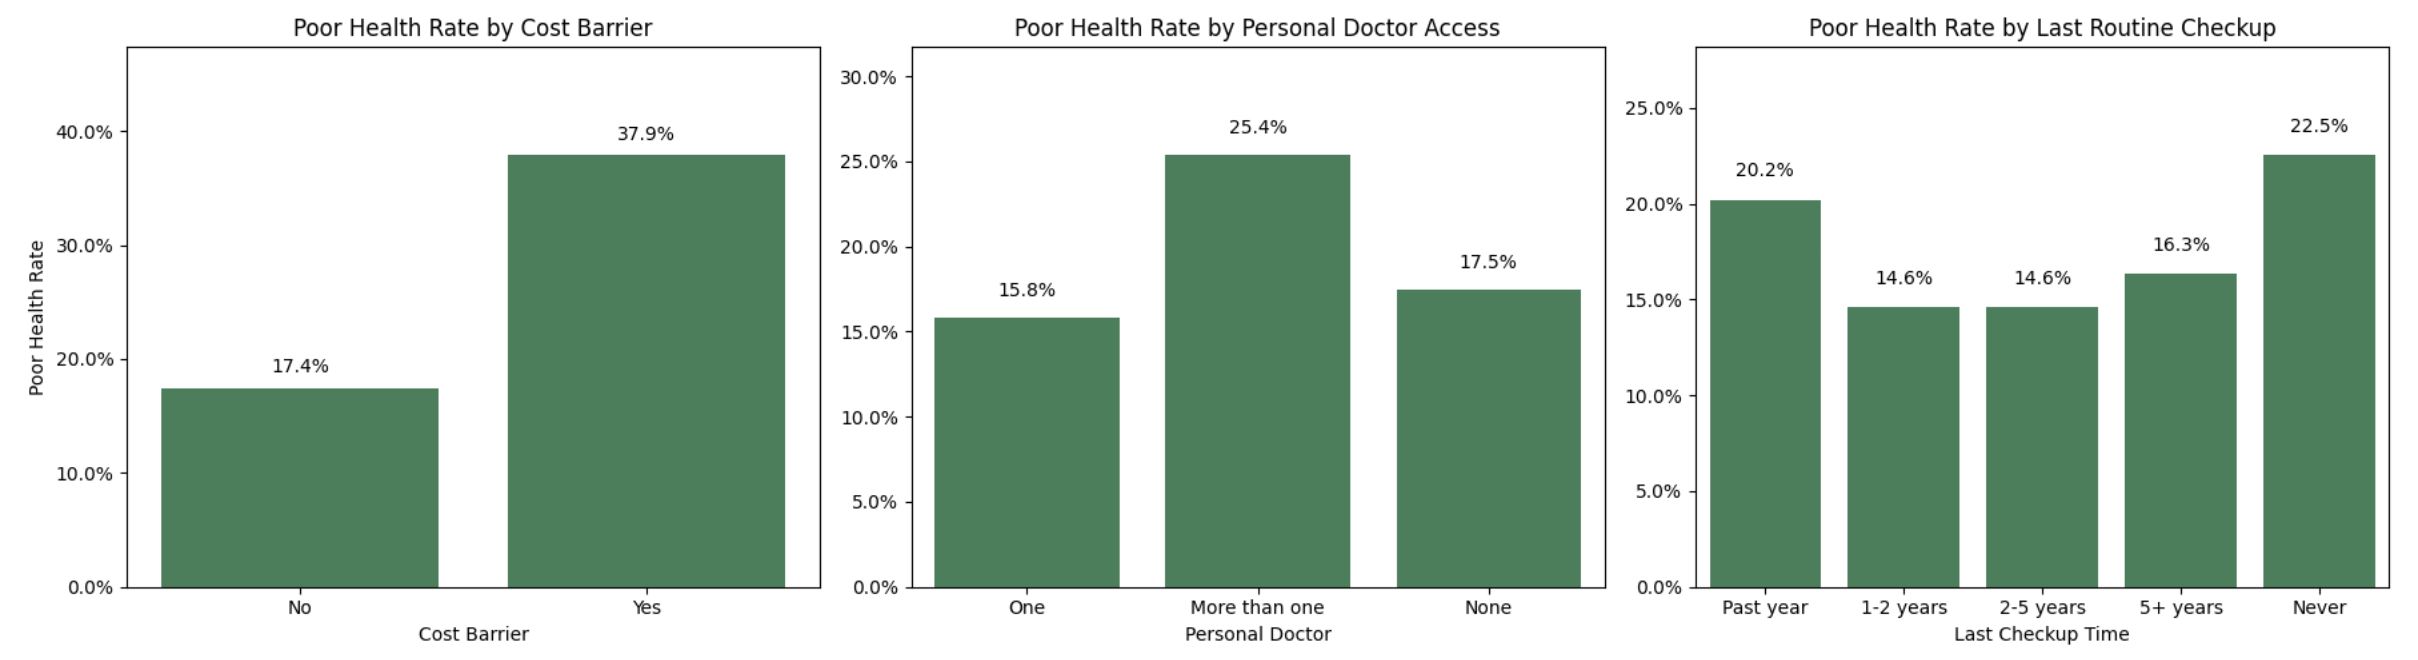
\includegraphics[width=\textwidth]{image/poor_health_by_healthcare_access.png}
    \caption{Poor-health rate by healthcare access variables.}
    \label{fig:poor_health_healthcare_access}
\end{figure}
Figure~\ref{fig:poor_health_healthcare_access} compares poor-health rates across three healthcare access variables. The clearest difference appears in the cost barrier variable. Respondents who reported being unable to see a doctor because of cost had a poor-health rate of 37.9\%, compared with 17.4\% for respondents without this barrier. This suggests that cost-related access problems were one of the strongest descriptive patterns in the EDA.

The personal doctor variable showed a different pattern. Respondents with more than one personal doctor had the highest poor-health rate at 25.4\%, while respondents with one personal doctor had a lower rate of 15.8\%. Respondents with no personal doctor had a rate of 17.5\%. This result may reflect the fact that people with more health needs are more likely to have multiple doctors, so this variable should be interpreted carefully.

For last routine checkup, respondents who never had a routine checkup had the highest poor-health rate at 22.5\%. Respondents with a checkup in the past year also had a relatively high rate at 20.2\%, while the 1--2 year and 2--5 year groups had lower rates at 14.6\%. Overall, these results show that healthcare access variables were related to differences in poor-health rates, especially the cost barrier variable.

\begin{figure}[H]
    \centering
    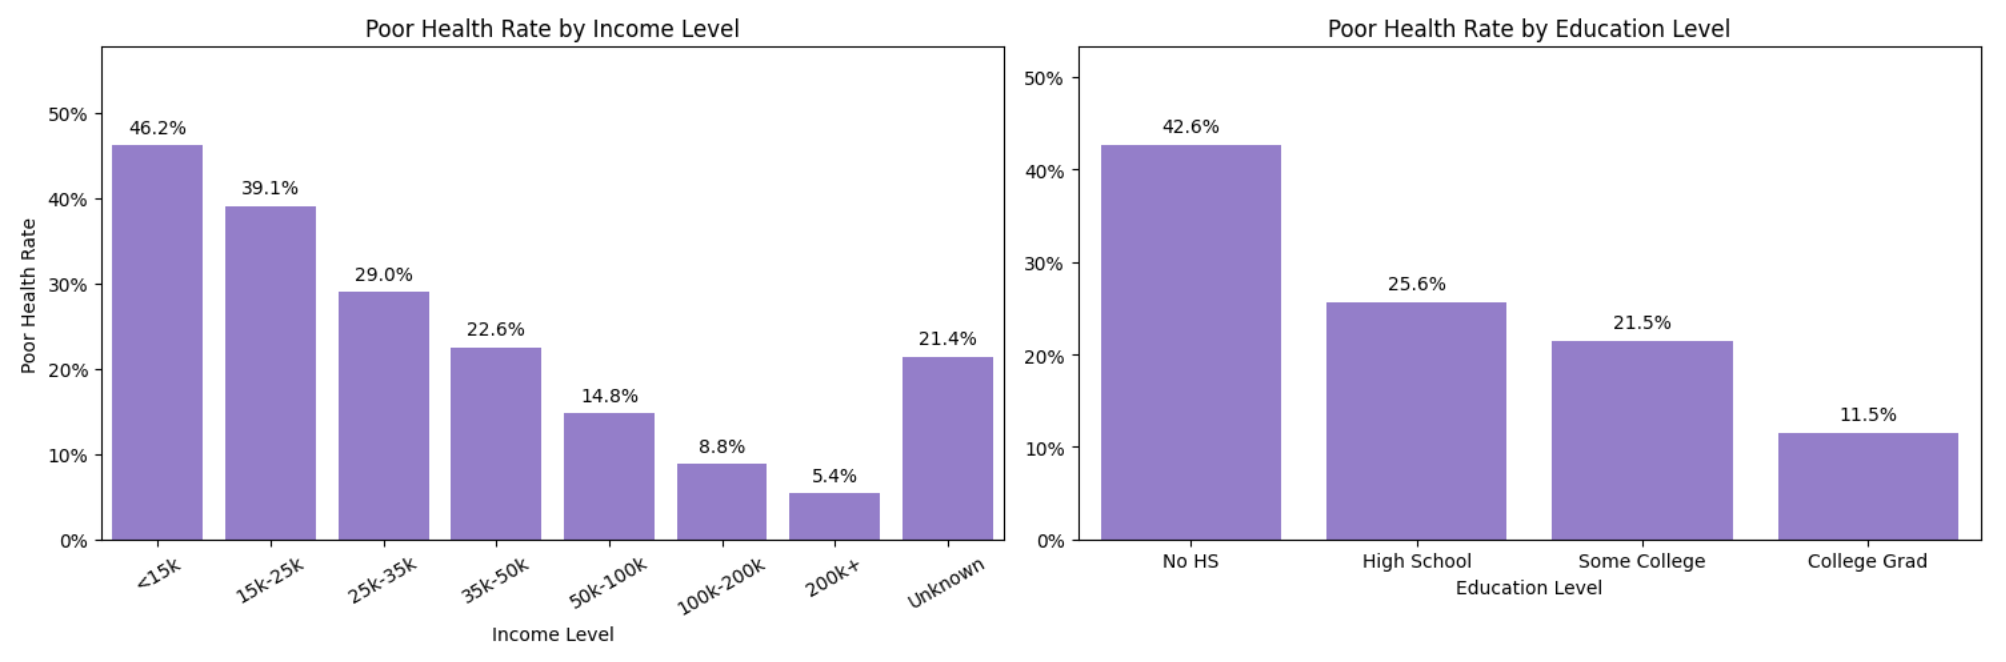
\includegraphics[width=0.80\textwidth]{image/poor_health_by_income_education.png}
    \caption{Poor-health rate by income level and education level.}
    \label{fig:poor_health_income_education}
\end{figure}
Figure~\ref{fig:poor_health_income_education} shows clear differences in poor-health rates across income and education groups. For income level, the poor-health rate generally decreased as income increased. Respondents with income below \$15,000 had the highest poor-health rate at 46.2\%, while respondents with income of \$200,000 or more had the lowest rate at 5.4\%. The unknown income group had a poor-health rate of 21.4\%, which was higher than the upper-income groups but lower than the lowest-income groups.

Education level showed a similar pattern. Respondents who did not graduate high school had the highest poor-health rate at 42.6\%. The rate was lower for high school graduates at 25.6\%, lower again for respondents with some college at 21.5\%, and lowest for college graduates at 11.5\%. These patterns suggest that socioeconomic variables were strongly related to differences in poor-health rates in the sample, which supports including income and education in the layered models.

\begin{figure}[H]
    \centering
    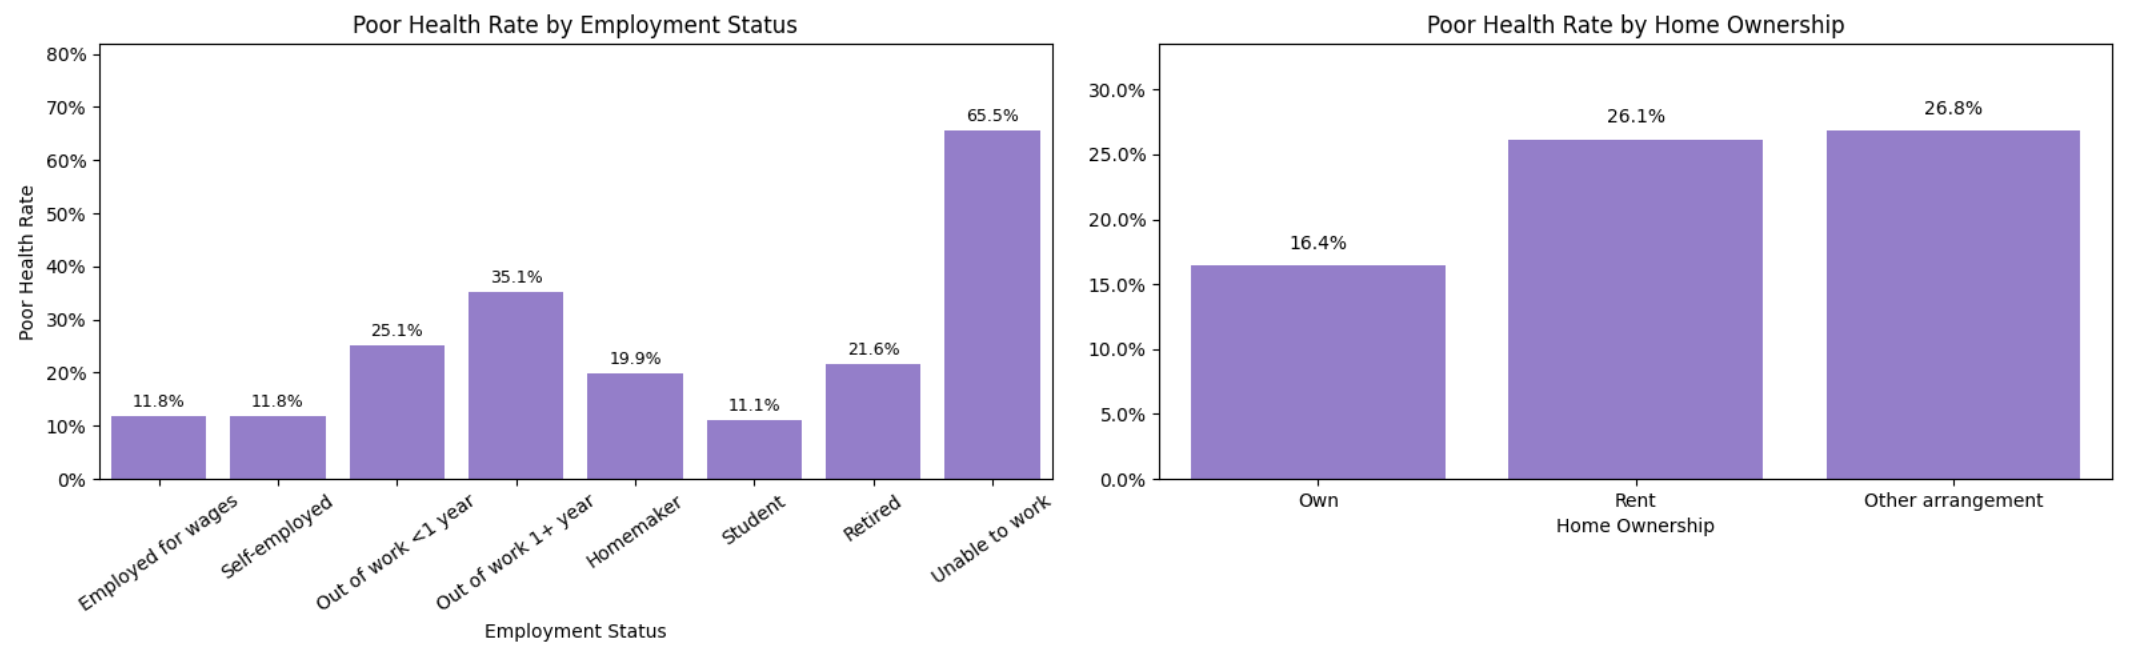
\includegraphics[width=0.80\textwidth]{image/poor_health_by_employment_homeownership.png}
    \caption{Poor-health rate by employment status and home ownership.}
    \label{fig:poor_health_employment_homeownership}
\end{figure}
Figure~\ref{fig:poor_health_employment_homeownership} shows poor-health rates by employment status and home ownership. The employment status variable showed one of the largest differences in poor-health rates. Respondents who were unable to work had the highest poor-health rate at 65.5\%. Respondents who were out of work for one year or more also had a higher rate at 35.1\%, while employed respondents and self-employed respondents both had much lower rates at 11.8\%. Students had the lowest rate at 11.1\%.

Home ownership also showed a clear difference. Respondents who owned their home had a poor-health rate of 16.4\%, while renters had a higher rate of 26.1\%. Respondents in other housing arrangements had a similar rate at 26.8\%. These results suggest that employment status and home ownership were useful socioeconomic variables for separating groups with different poor-health rates. However, the ``unable to work'' group should be interpreted carefully because this category may partly reflect existing health limitations.

\begin{figure}[H]
    \centering
    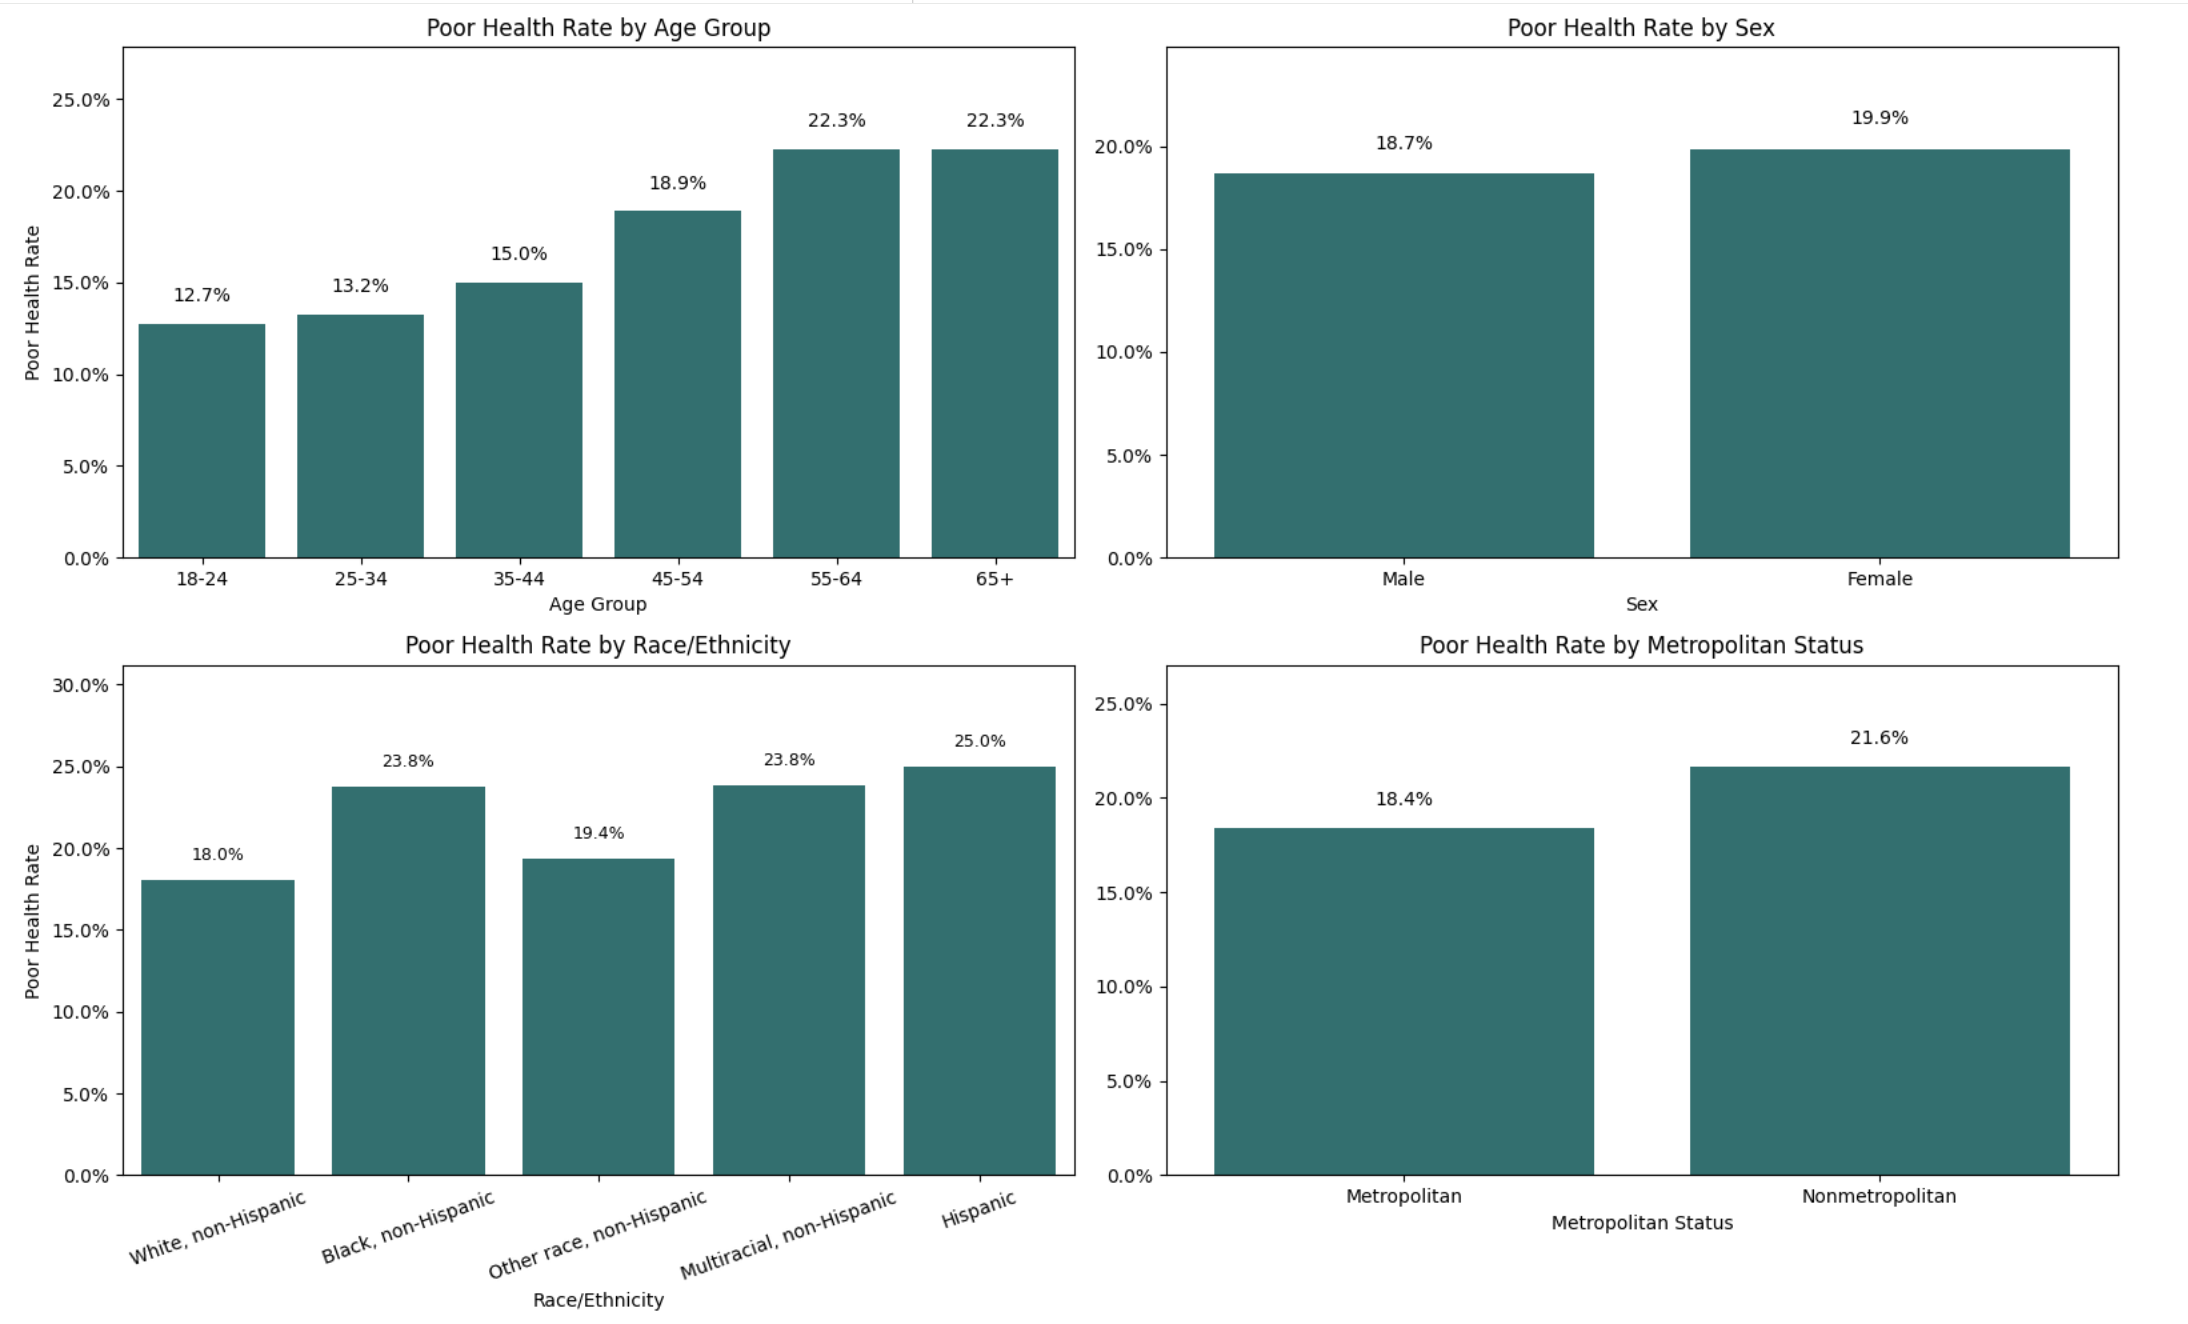
\includegraphics[width=0.75\textwidth]{image/poor_health_by_demographics.png}
    \caption{Poor-health rate by demographic variables.}
    \label{fig:poor_health_demographics}
\end{figure}
Figure~\ref{fig:poor_health_demographics} shows poor-health rates across demographic groups. Age group showed a clear increasing pattern. Respondents aged 18--24 had the lowest poor-health rate at 12.7\%, while the rate increased to 22.3\% for both the 55--64 and 65+ groups. This suggests that age group was related to differences in self-reported poor health.

Sex showed only a small difference in poor-health rates. Male respondents had a poor-health rate of 18.7\%, while female respondents had a rate of 19.9\%. This difference was much smaller than the differences seen for income, education, employment status, and cost barrier.

Race/ethnicity and metropolitan status also showed some differences. Hispanic respondents had the highest poor-health rate at 25.0\%, while White non-Hispanic respondents had a lower rate at 18.0\%. Black non-Hispanic and multiracial non-Hispanic respondents both had rates of 23.8\%. For metropolitan status, nonmetropolitan respondents had a higher poor-health rate at 21.6\%, compared with 18.4\% for metropolitan respondents. Overall, these demographic variables showed some group differences, but the earlier socioeconomic and healthcare access variables showed larger differences in poor-health rates.

\begin{figure}[!htbp]
    \centering
    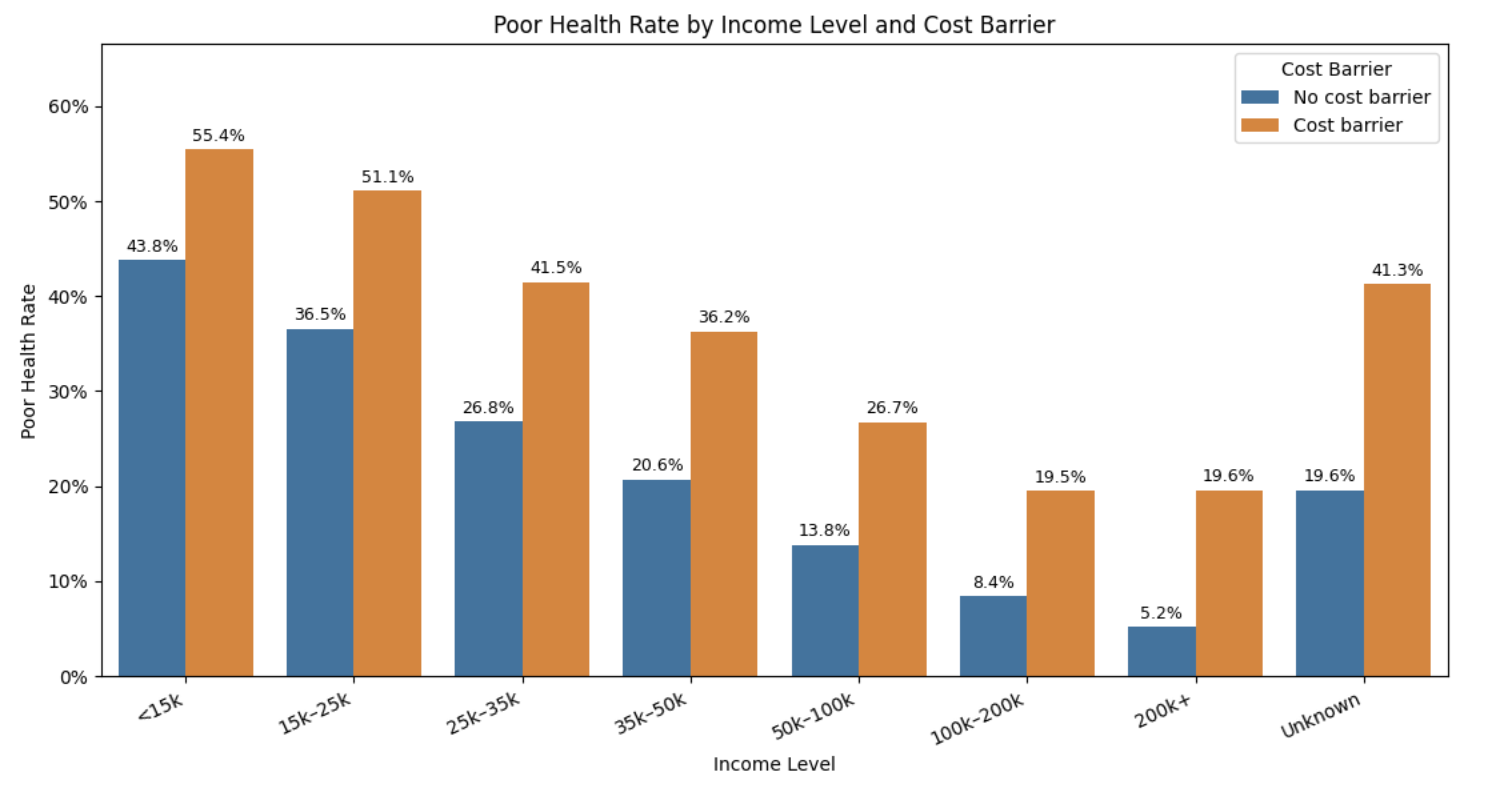
\includegraphics[width=0.90\textwidth]{image/poor_health_by_income_cost_barrier.png}
    \caption{Poor-health rate by income level and cost barrier status.}
    \label{fig:poor_health_income_cost_barrier}
\end{figure}
Figure~\ref{fig:poor_health_income_cost_barrier} compares poor-health rates by income level and cost barrier status. Across every income group, respondents with a cost barrier had a higher poor-health rate than respondents without a cost barrier. The difference was clear even in higher-income groups. For example, among respondents with income of \$200,000 or more, the poor-health rate was 5.2\% for those without a cost barrier, compared with 19.6\% for those with a cost barrier.

The figure also shows that income level still mattered within both cost-barrier groups. In general, lower-income groups had higher poor-health rates than higher-income groups. The highest rate appeared in the group with income below \$15,000 and a cost barrier, where 55.4\% reported poor health. This pattern suggests that income level and cost-related healthcare barriers were both useful for describing differences in poor-health rates in the sample.

\begin{figure}[H]
    \centering
    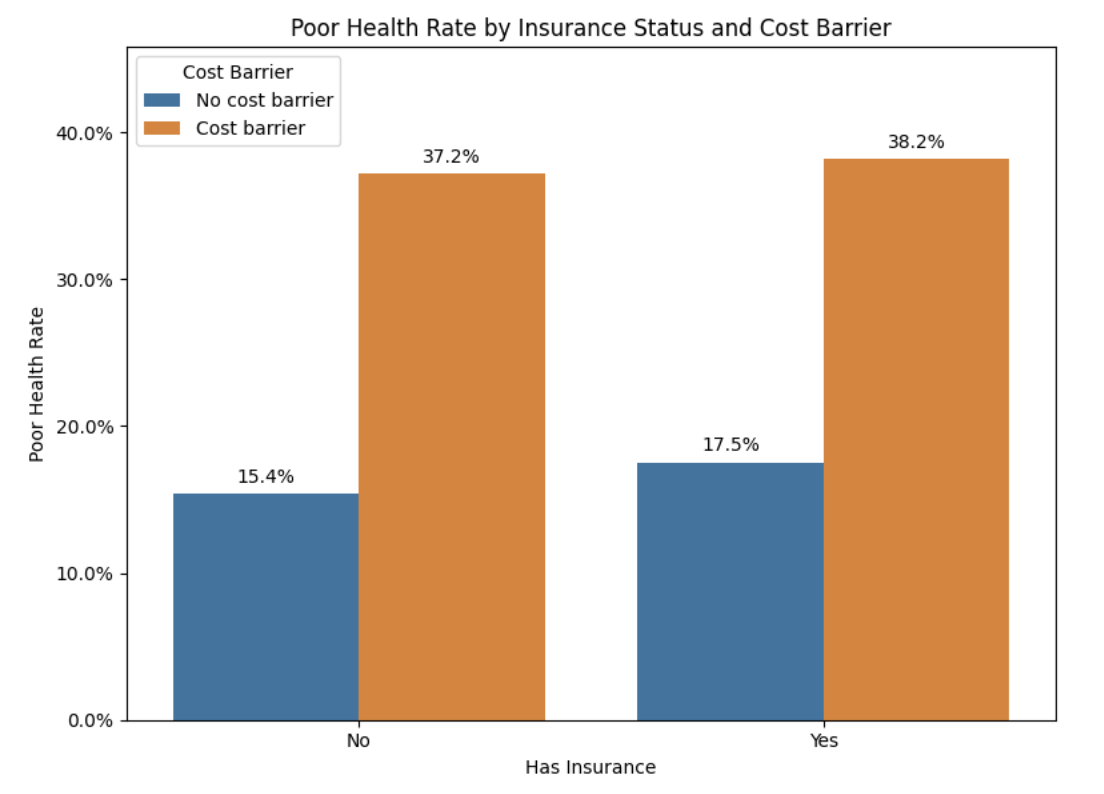
\includegraphics[width=0.70\textwidth]{image/poor_health_by_insurance_cost_barrier.png}
    \caption{Poor-health rate by insurance status and cost barrier status.}
    \label{fig:poor_health_insurance_cost_barrier}
\end{figure}
Figure~\ref{fig:poor_health_insurance_cost_barrier} compares poor-health rates by insurance status and cost barrier status. In both insurance groups, respondents with a cost barrier had much higher poor-health rates than respondents without a cost barrier. Among uninsured respondents, the poor-health rate was 15.4\% for those without a cost barrier and 37.2\% for those with a cost barrier. Among insured respondents, the rate was 17.5\% without a cost barrier and 38.2\% with a cost barrier.

This pattern shows that cost-related access problems were important even when insurance status was considered. The poor-health rate was very similar for respondents with a cost barrier, whether they had insurance or not. This suggests that insurance status alone did not fully capture healthcare access problems in the sample, which supports including both insurance information and cost barrier in the models.

\begin{figure}[H]
    \centering
    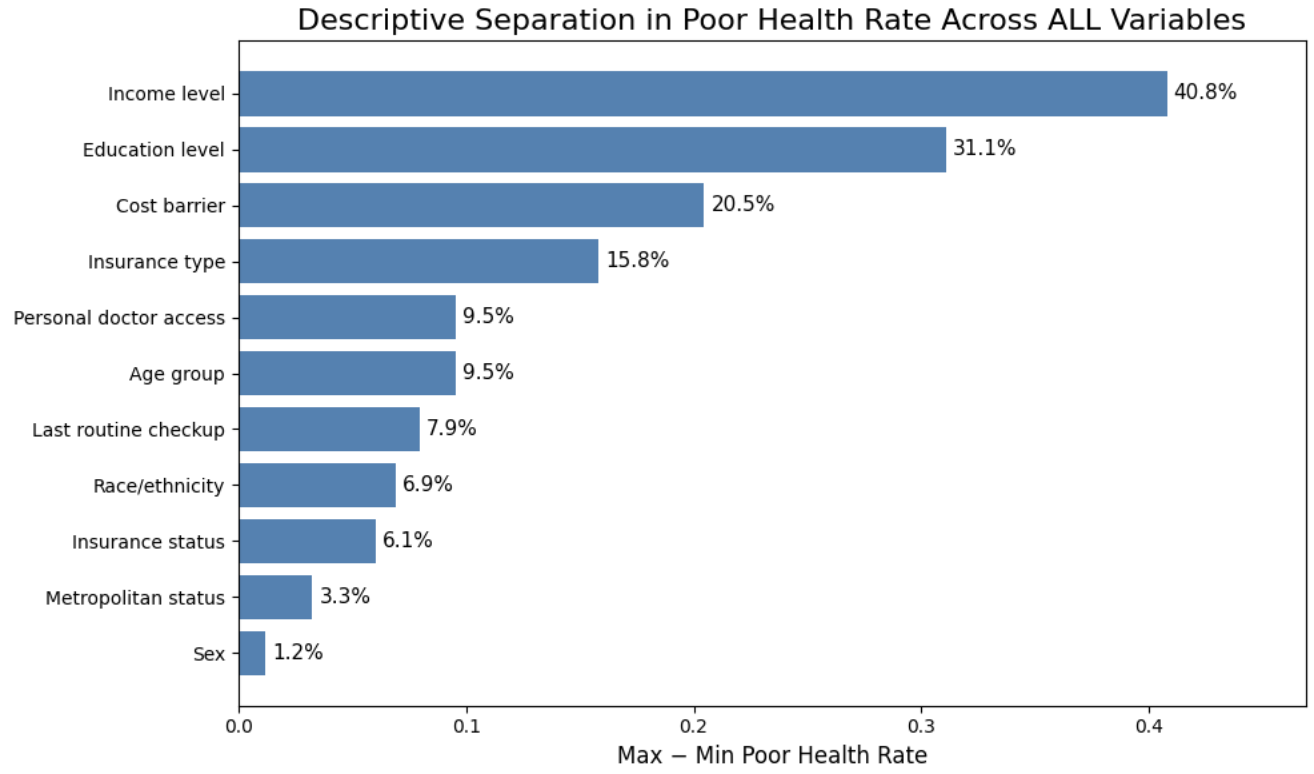
\includegraphics[width=0.75\textwidth]{image/descriptive_separation_all_variables.png}
    \caption{Descriptive separation in poor-health rates across selected variables.}
    \label{fig:descriptive_separation}
\end{figure}
Figure~\ref{fig:descriptive_separation} summarizes the spread in poor-health rates across the selected variables. The value for each variable represents the difference between the highest and lowest poor-health rate across its categories. Income level showed the largest separation at 40.8\%, followed by education level at 31.1\%. Cost barrier also showed a clear separation at 20.5\%, while insurance type showed a smaller but still visible separation at 15.8\%.

Other variables showed smaller differences. Personal doctor access and age group both had a separation of 9.5\%, while last routine checkup had a separation of 7.9\%. Race/ethnicity, insurance status, metropolitan status, and sex showed smaller separations. Overall, this summary supports the earlier EDA patterns: socioeconomic variables, especially income and education, showed the largest differences in poor-health rates, followed by cost-related healthcare access.

\begin{figure}[!htbp]
    \centering
    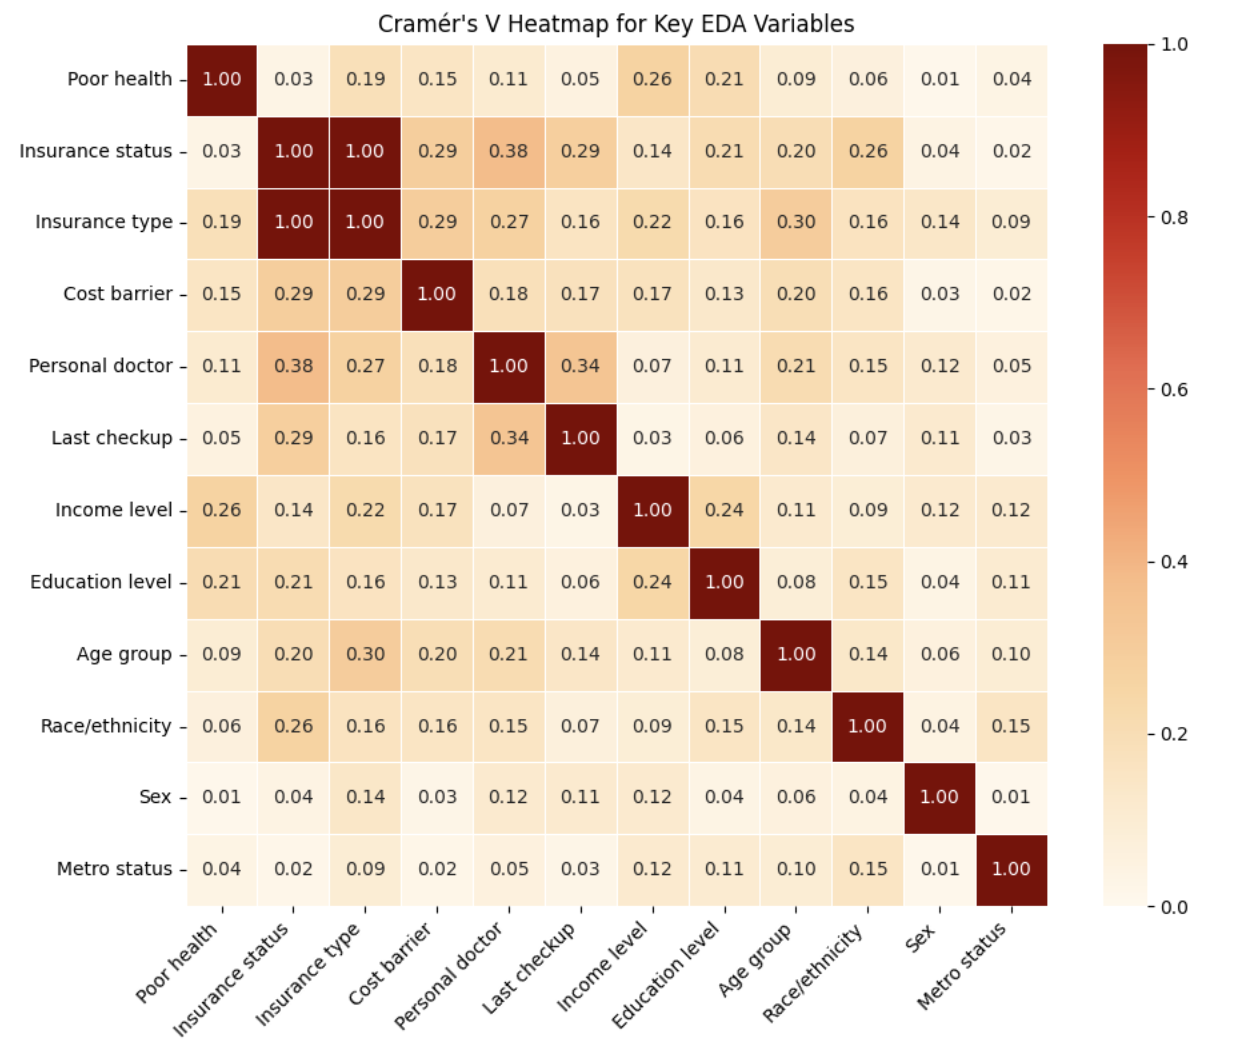
\includegraphics[width=0.80\textwidth]{image/cramers_v_heatmap.png}
    \caption{Cramér's V heatmap for selected categorical variables.}
    \label{fig:cramers_v_heatmap}
\end{figure}
Figure~\ref{fig:cramers_v_heatmap} shows the Cramér's V values among the selected categorical variables. For the relationship with \texttt{poor\_health}, income level had the highest value at 0.26, followed by education level at 0.21, insurance type at 0.19, and cost barrier at 0.15. These values are not very high, but they show that these variables had stronger categorical associations with \texttt{poor\_health} than variables such as sex, metropolitan status, or last routine checkup.

The heatmap also shows that some predictors were related to each other. Insurance status and insurance type had a value of 1.00 because they contain overlapping insurance information. Personal doctor access and insurance status also showed a moderate relationship at 0.38, and personal doctor access and last routine checkup had a value of 0.34. These patterns were useful to check before modeling because they show where some predictor information may overlap. Overall, the heatmap supports the earlier EDA results: income, education, insurance type, and cost barrier were among the more useful variables for understanding differences in poor-health rates, while no single variable fully explained the outcome by itself.

Overall, the EDA results show that poor-health rates were not evenly distributed across the selected non-clinical variables. The largest differences appeared in socioeconomic variables, especially income level, education level, and employment status. Healthcare access also showed clear patterns, especially for respondents who reported a cost barrier. Insurance information was useful, but insurance status alone did not explain the full pattern because cost barriers still appeared among both insured and uninsured respondents. These EDA findings supported the layered model design by showing that insurance, healthcare access, and socioeconomic variables each provided useful descriptive information for predicting \texttt{poor\_health}.

\subsection{Layered Model Comparison}

\begin{table}[H]
\centering
\caption{3-Fold Cross-Validation Performance Across Layered Models}
\label{tab:layered_cv_results}
\begin{tabular}{llrr}
\toprule
Model Type & Layered Model & F1 Score & ROC-AUC \\
\midrule
Logistic Regression & Model 1 & 0.384 & 0.618 \\
Logistic Regression & Model 2 & 0.398 & 0.684 \\
Logistic Regression & Model 3 & 0.470 & 0.763 \\
Logistic Regression & Model 4 & 0.477 & 0.767 \\
\midrule
Random Forest & Model 1 & 0.384 & 0.618 \\
Random Forest & Model 2 & 0.399 & 0.685 \\
Random Forest & Model 3 & 0.451 & 0.723 \\
Random Forest & Model 4 & 0.410 & 0.690 \\
\midrule
XGBoost & Model 1 & 0.384 & 0.618 \\
XGBoost & Model 2 & 0.399 & 0.685 \\
XGBoost & Model 3 & 0.467 & 0.762 \\
XGBoost & Model 4 & 0.470 & 0.764 \\
\bottomrule
\end{tabular}
\end{table}
The cross-validation results show that adding socioeconomic variables in Model 3 produced the largest improvement across the layered models. Model 4 gave the best performance for Logistic Regression and XGBoost, but the improvement from Model 3 to Model 4 was small. For Random Forest, Model 3 performed better than Model 4. Overall, the results suggest that socioeconomic variables added the most useful predictive information, while demographic variables provided only limited additional improvement.

\begin{figure}[H]
    \centering
    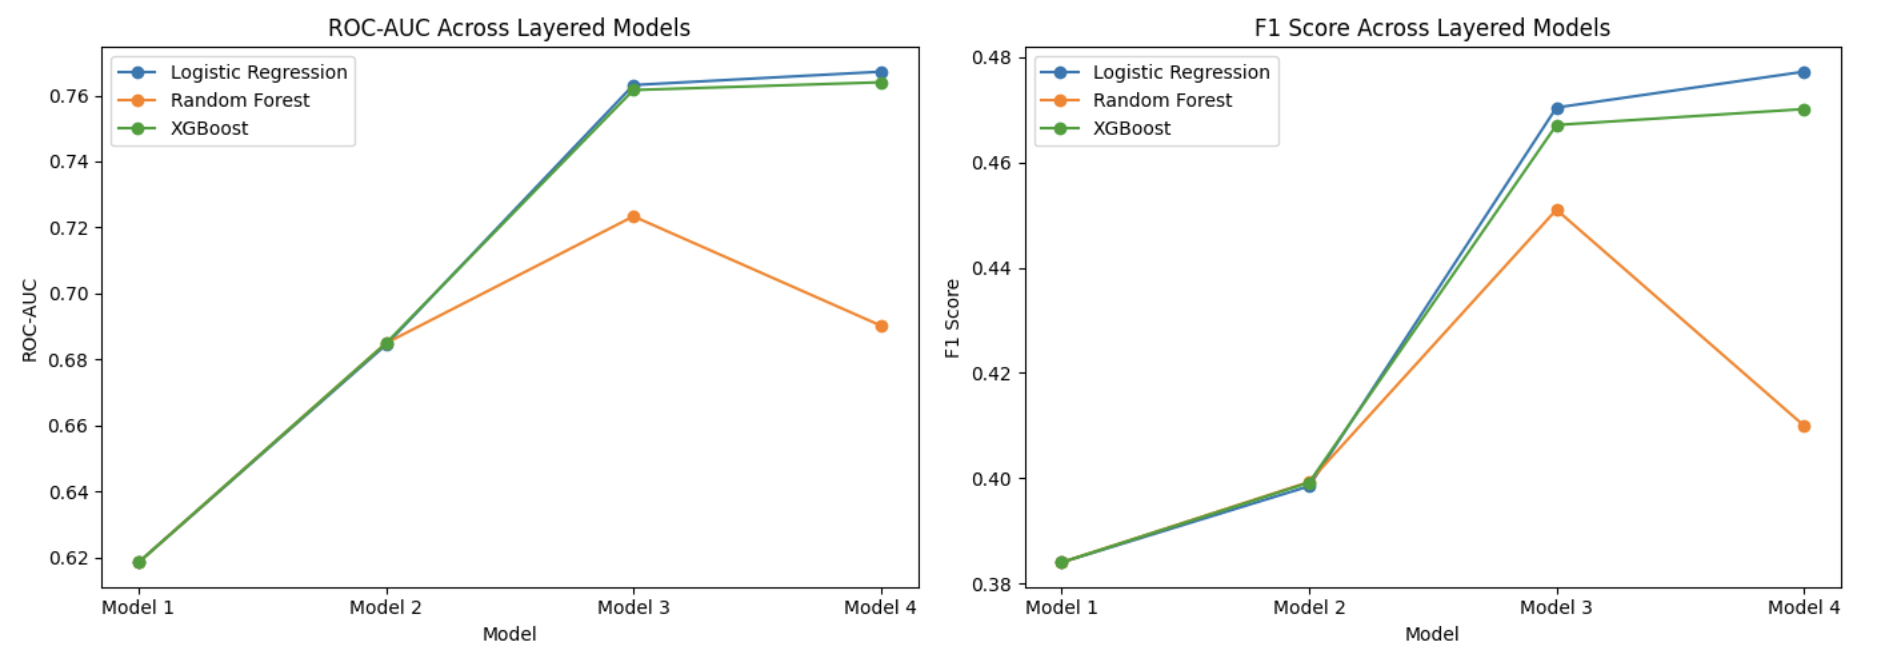
\includegraphics[width=0.70\textwidth]{image/layered_model_comparison.png}
    \caption{Cross-validation ROC-AUC and F1 score across layered model designs.}
    \label{fig:layered_model_comparison}
\end{figure}
Figure~\ref{fig:layered_model_comparison} shows how ROC-AUC and F1 score changed as more predictor groups were added to the models. Model 1, which only used insurance information, had the lowest performance for all three algorithms. After healthcare access variables were added in Model 2, both ROC-AUC and F1 score increased slightly.

The largest improvement happened from Model 2 to Model 3, when socioeconomic variables were added. This pattern is clear for Logistic Regression and XGBoost, where both ROC-AUC and F1 score increased sharply. Random Forest also improved from Model 2 to Model 3, but its scores stayed lower than Logistic Regression and XGBoost.

Model 4 added demographic variables. For Logistic Regression and XGBoost, Model 4 gave only a small additional improvement over Model 3. For Random Forest, Model 4 performed worse than Model 3 in both ROC-AUC and F1 score. Overall, this figure suggests that socioeconomic variables added the most useful predictive information, while demographic variables added less additional value.

\subsection{Final Test-Set Model Performance}
After comparing the layered models with cross-validation, we evaluated the final Model 4 versions on the held-out test set. Model 4 used the full set of non-clinical predictors, including insurance information, healthcare access variables, socioeconomic variables, and demographic variables. Table~\ref{tab:model4_test_results} summarizes the final test-set performance for Logistic Regression, Random Forest, and XGBoost.

\begin{table}[H]
\centering
\caption{Final Test-Set Performance for Model 4}
\label{tab:model4_test_results}
\begin{tabular}{lrrrrr}
\toprule
Model & Accuracy & Precision & Recall & F1 Score & ROC-AUC \\
\midrule
Logistic Regression & 0.719 & 0.373 & 0.669 & 0.479 & 0.767 \\
Random Forest & 0.744 & 0.373 & 0.477 & 0.418 & 0.693 \\
XGBoost & 0.711 & 0.366 & 0.675 & 0.474 & 0.765 \\
\bottomrule
\end{tabular}
\end{table}

Logistic Regression and XGBoost had very similar test-set performance. Logistic Regression had the highest F1 score at 0.479 and the highest ROC-AUC at 0.767. XGBoost had the highest recall at 0.675, which means it identified slightly more true poor-health cases than Logistic Regression. However, the difference between Logistic Regression and XGBoost was very small across the main metrics.

Random Forest had the highest accuracy at 0.744, but its recall was much lower at 0.477. Since this project focuses on identifying respondents who reported poor health, recall is important because it shows how many true poor-health cases the model found. Random Forest also had the lowest F1 score and ROC-AUC, which suggests that its higher accuracy mainly came from better performance on the larger non-poor-health group. Overall, Logistic Regression and XGBoost performed better than Random Forest for the goal of identifying poor-health respondents.

\begin{figure}[H]
    \centering
    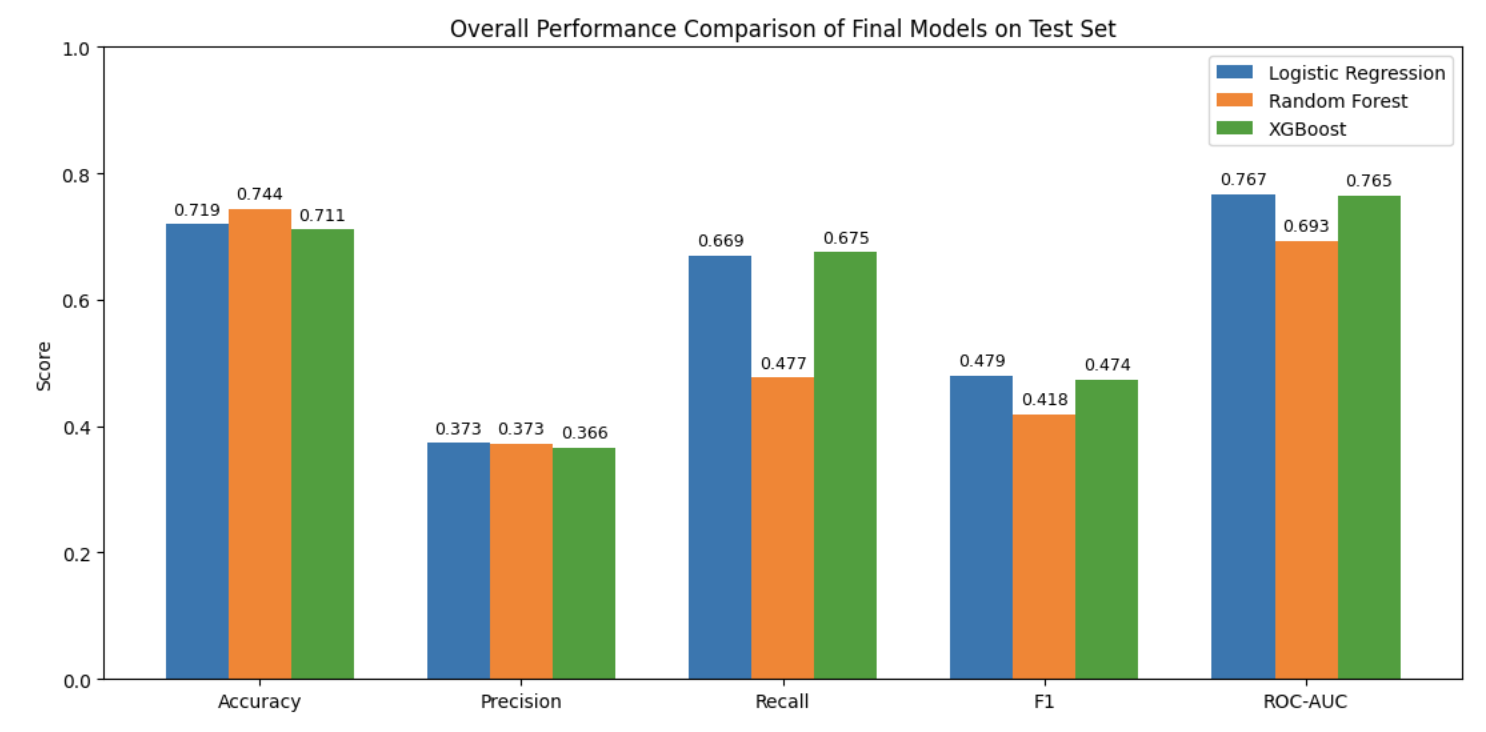
\includegraphics[width=0.70\textwidth]{image/final_model_performance.png}
    \caption{Overall performance comparison of final Model 4 classifiers on the test set.}
    \label{fig:final_model_performance}
\end{figure}
Figure~\ref{fig:final_model_performance} gives a visual comparison of the final test-set metrics. Logistic Regression and XGBoost performed very similarly, with Logistic Regression having the highest F1 score and ROC-AUC and XGBoost having the highest recall. Random Forest had the highest accuracy, but its recall and ROC-AUC were lower than the other two models. Since the goal was to identify poor-health respondents, the recall, F1 score, and ROC-AUC results were more important than accuracy alone.

\begin{figure}[H]
    \centering
    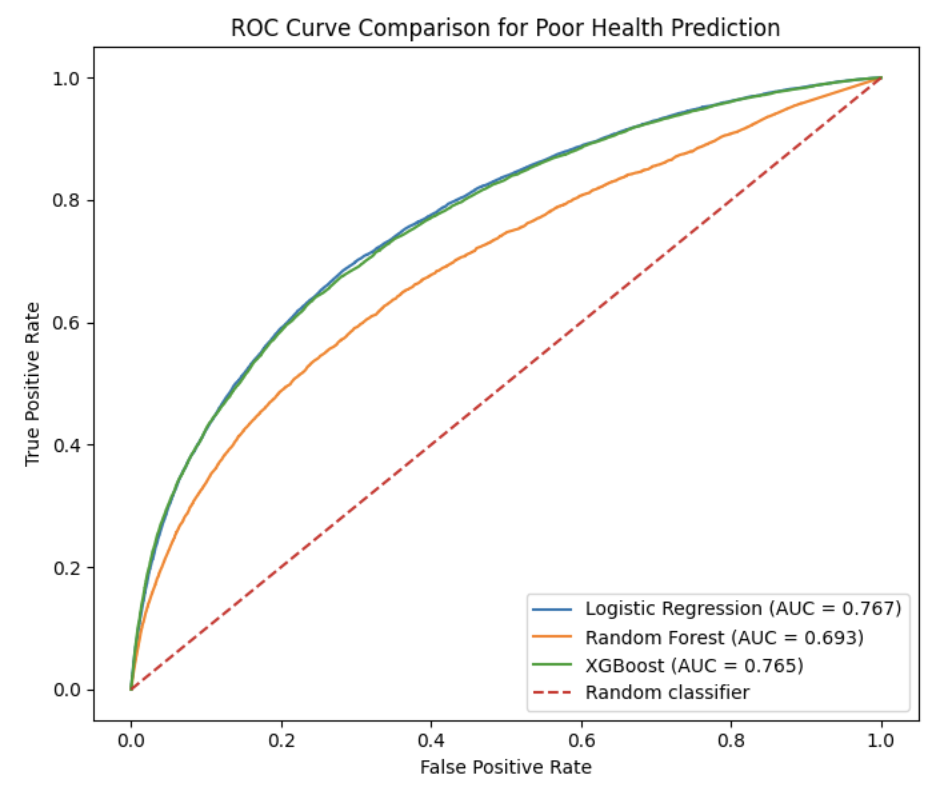
\includegraphics[width=0.78\textwidth]{image/roc_curve_comparison.png}
    \caption{ROC curve comparison of final Model 4 classifiers on the test set.}
    \label{fig:roc_curve_comparison}
\end{figure}
Figure~\ref{fig:roc_curve_comparison} compares the ROC curves for the three final Model 4 classifiers. Logistic Regression and XGBoost had very similar curves, and both stayed above the Random Forest curve across most of the plot. Logistic Regression had the highest ROC-AUC at 0.767, while XGBoost was very close at 0.765. This shows that the two models had almost the same ability to rank respondents by predicted poor-health risk.

Random Forest had a lower ROC-AUC at 0.693, and its curve stayed closer to the random classifier line than the other two models. This means that Random Forest had weaker separation between respondents who reported poor health and those who did not. Overall, the ROC curve supports the earlier metric comparison: Logistic Regression and XGBoost performed better than Random Forest on the final test set.

\subsection{Model Interpretation}

\begin{figure}[!htbp]
    \centering
    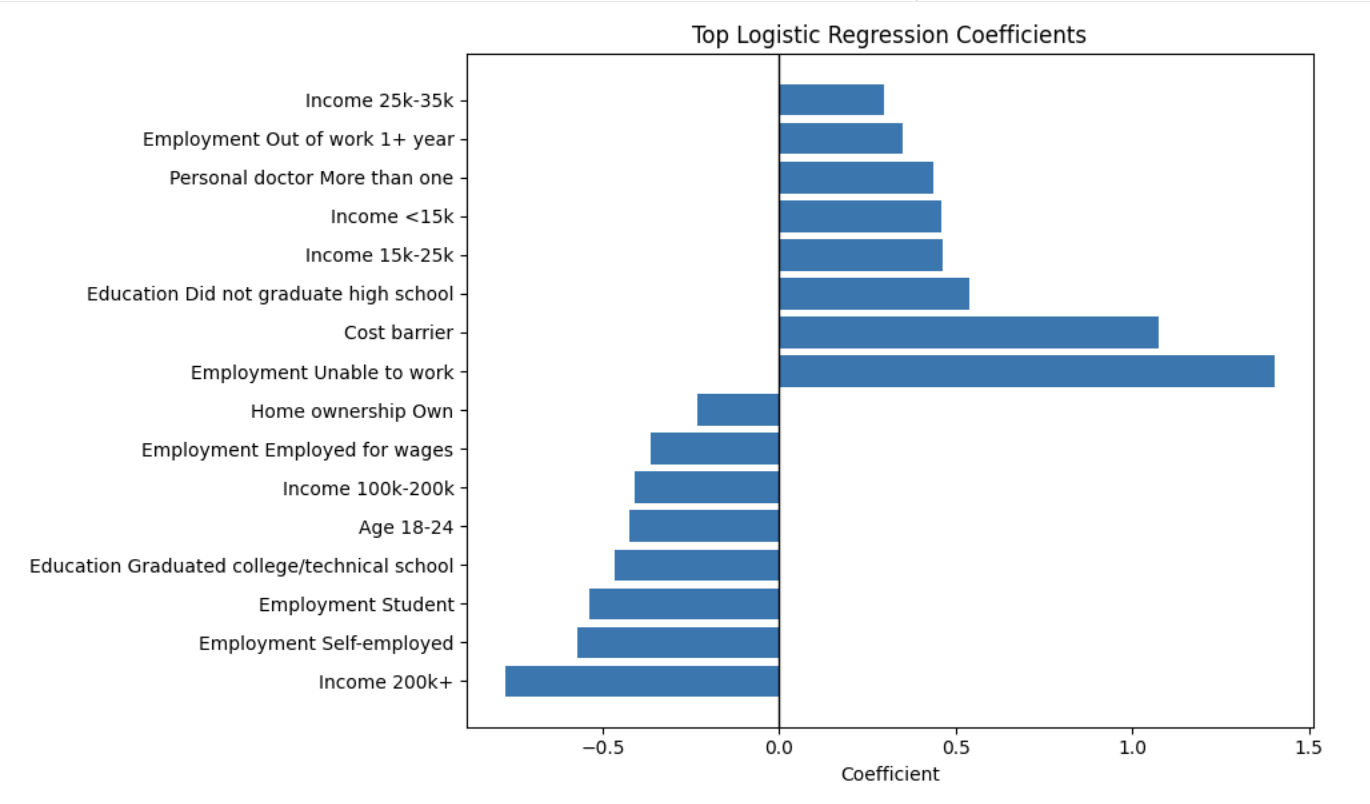
\includegraphics[width=0.75\textwidth]{image/lr_coefficients.png}
    \caption{Top positive and negative Logistic Regression coefficients.}
    \label{fig:lr_coefficients}
\end{figure}
Figure~\ref{fig:lr_coefficients} shows the largest positive and negative coefficients from the Logistic Regression model. Positive coefficients are related to a higher predicted probability of reporting poor health, while negative coefficients are related to a lower predicted probability. The largest positive coefficient was for the ``Unable to work'' employment category, followed by cost barrier. This means that these categories were strongly related to higher predicted poor-health risk in the model.

Several low-income and lower-education categories also had positive coefficients, including income below \$15,000, income between \$15,000 and \$25,000, and not graduating high school. This pattern is consistent with the EDA results, where lower income and lower education groups had higher poor-health rates. On the negative side, income of \$200,000 or more, being self-employed, being a student, and graduating college or technical school were related to lower predicted poor-health risk.

These coefficients should be interpreted as predictive relationships, not causal effects. 

\begin{figure}[H]
    \centering
    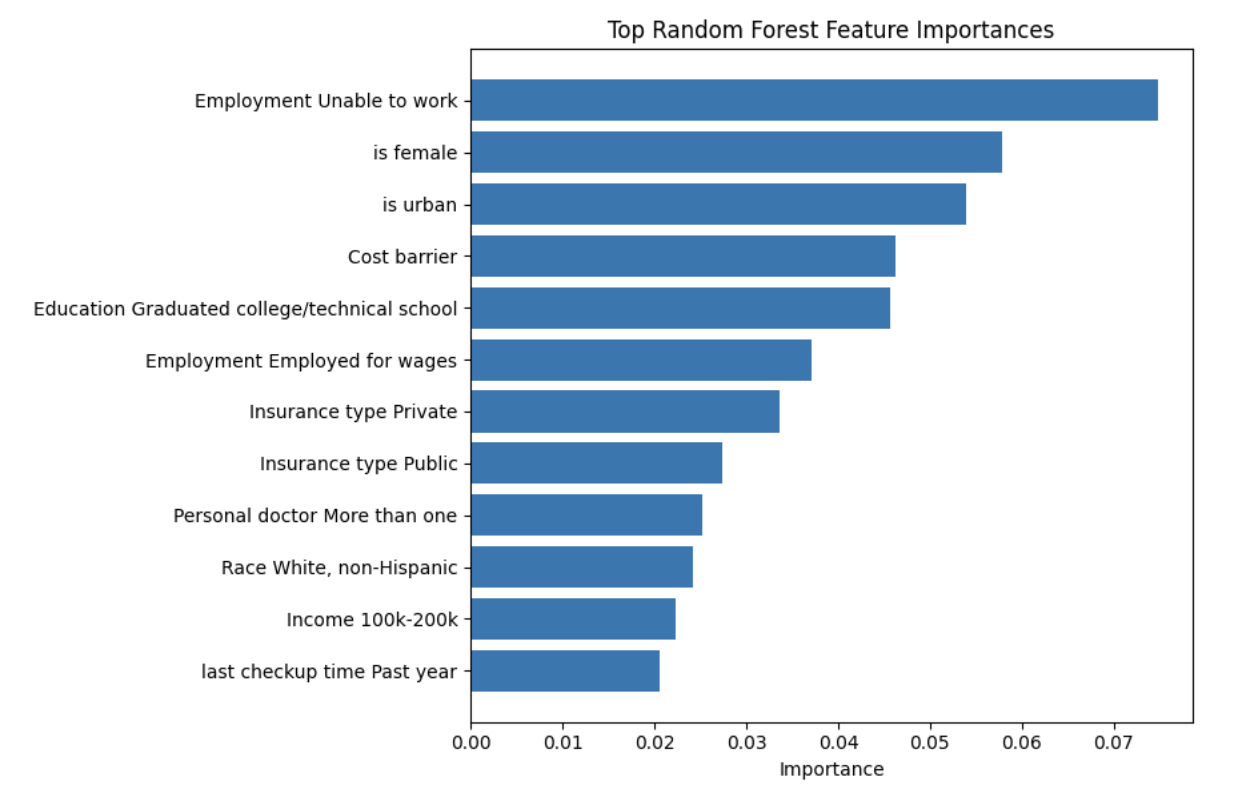
\includegraphics[width=0.75\textwidth]{image/rf_feature_importance.png}
    \caption{Top Random Forest feature importances.}
    \label{fig:rf_feature_importance}
\end{figure}
Figure~\ref{fig:rf_feature_importance} shows the top features from the Random Forest model. The most important feature was the ``Unable to work'' employment category. Cost barrier also appeared among the top features, which is consistent with the EDA results and the Logistic Regression coefficients. Several other features from employment status, education, insurance type, personal doctor access, race/ethnicity, income, and last checkup time also appeared in the top list.

Unlike Logistic Regression coefficients, Random Forest feature importance does not show whether a feature is related to higher or lower predicted poor-health risk. It only shows which features were used more by the model to make predictions. For this reason, these values should be interpreted as model importance rather than causal effects. 

\begin{figure}[!htbp]
    \centering
    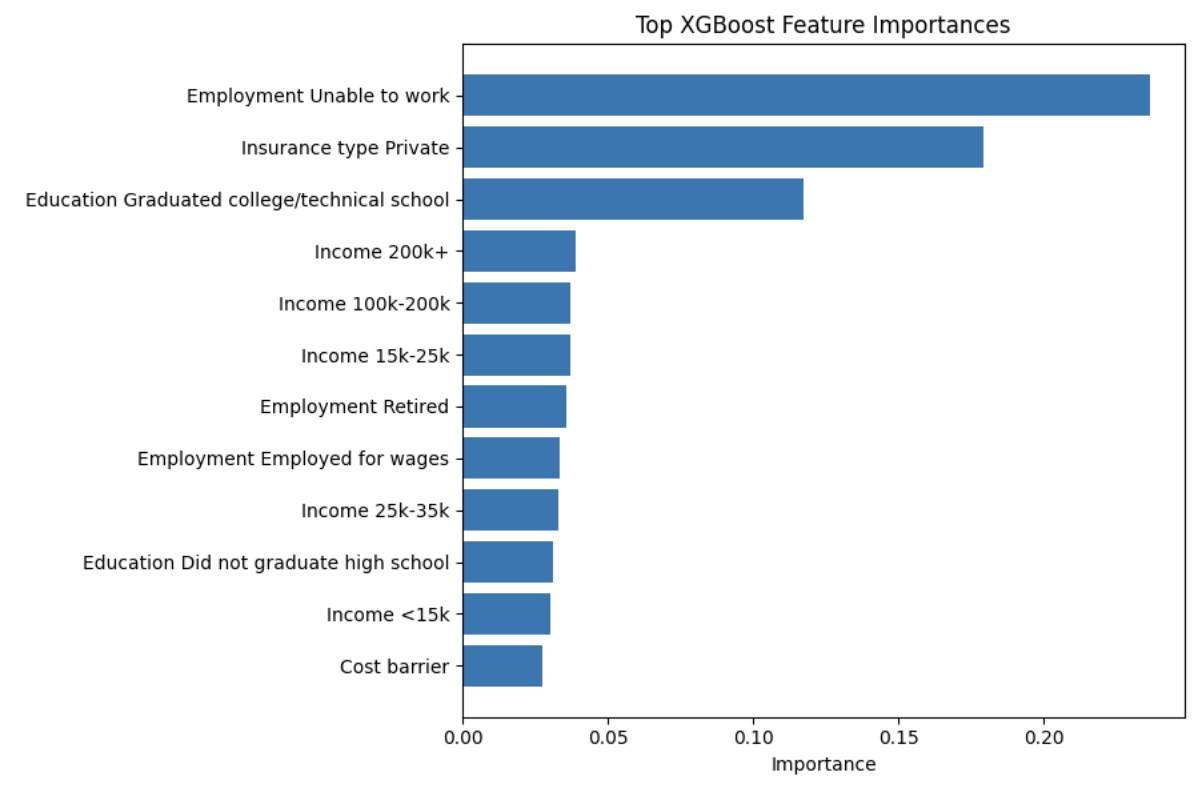
\includegraphics[width=0.75\textwidth]{image/xgb_feature_importance.png}
    \caption{Top XGBoost feature importances.}
    \label{fig:xgb_feature_importance}
\end{figure}
Figure~\ref{fig:xgb_feature_importance} shows the top feature importances from the XGBoost model. The most important feature was again the ``Unable to work'' employment category. This matches the Logistic Regression and Random Forest results, where this category also appeared as one of the strongest predictors. Insurance type private and graduating college or technical school were also among the top features, followed by several income and employment categories.

The XGBoost importance plot shows that the model used a mix of employment, insurance, education, and income-related features to make predictions. Cost barrier also appeared in the top list, but it was less important in XGBoost than in the Logistic Regression and Random Forest results. Like the Random Forest importance values, XGBoost feature importance does not show the direction of the relationship. It only shows which features were more useful for the model's prediction. Therefore, these results should be interpreted as predictive importance, not causal effects.

Overall, the model interpretation results matched the earlier EDA results. Employment status, especially the ``Unable to work'' group, was important in all three models. Cost barrier, income, education, and insurance type also appeared often in the coefficient and feature importance plots. This shows that the models mainly used socioeconomic and healthcare access information to predict \texttt{poor\_health}. However, these patterns should not be read as causal effects. The ``Unable to work'' group should be interpreted carefully because it may already reflect health problems.

\subsection{Final Model Selection}
Based on the test-set results, we selected Logistic Regression as the final model. Logistic Regression had the highest ROC-AUC at 0.767 and the highest F1 score at 0.479. Its recall was also high at 0.669, which was close to XGBoost's recall of 0.675. This means that Logistic Regression was able to identify many poor-health cases while keeping a slightly better balance between precision and recall.

XGBoost performed very similarly to Logistic Regression and had the highest recall. However, its F1 score and ROC-AUC were slightly lower than Logistic Regression. Random Forest had the highest accuracy, but its recall and ROC-AUC were much lower. Since the goal of this project was to identify respondents who reported poor health, accuracy alone was not enough to choose the final model.

Logistic Regression was also easier to interpret than the two tree-based models. Its coefficients helped show which variables were related to higher or lower predicted poor-health risk. For these reasons, Logistic Regression was selected as the final model for this project.

\section{Discussion}

\subsection{Summary of Main Findings}
Using nonclinical factors, this project aims to identify adults in the 2024 BRFSS dataset who may have a higher risk of poor health. The results show that poor health is not evenly distributed, and the model cannot accurately identify adults at risk of poor health by only looking at accuracy. As shown in Figure~\ref{fig:poor_health_distribution}, most respondents were classified as not poor health, up to 80.7 percent, while only 19.3 percent were classified as poor health. Therefore, accuracy alone can be misleading when evaluating the classification of poor health individuals. Recall, F1 score, and ROC-AUC are also important evaluation metrics.

Economic variables show the most obvious differences in poor health risk. As shown in Figure~\ref{fig:descriptive_separation} , income level has the strongest descriptive separation, up to 40.8 percent, followed by education level and cost barrier. This suggests that income status, education level, and healthcare cost burden are more useful for distinguishing adults at risk of poor health. The EDA also found that even among respondents who had insurance, those with cost barriers still had a high poor health rate. This shows that having insurance does not always mean healthcare is affordable, and these respondents may still have a high risk of poor health.
The layered model comparison also supports the findings from the EDA. As shown in Figure 12, Model 1, which only used insurance type, had the weakest performance. This means the model could not accurately identify adults at risk of poor health. The largest improvement happened after adding socioeconomic variables in Model 3, which also supports that adding these economic factors can help the model better identify adults at risk of poor health.

Among the three models in this project, Logistic Regression and XGBoost best fit the goal of this project. Although Figure~\ref{fig:final_model_performance} shows that Random Forest had the highest accuracy, its recall was low, meaning that the Random Forest model missed many real poor-health respondents. Logistic Regression and XGBoost performed better for this project.

\subsection{Interpretation of Results}
Adults at risk of poor health are not determined only by whether they have insurance or not. As shown in Figure~\ref{fig:descriptive_separation}, income level, education level, and cost barrier show clear differences in poor health rate. Although people without insurance have a higher poor health rate than people with insurance, the effect of insurance status is smaller compared with income, education, and cost barrier. Insurance is important, but it cannot fully determine whether adults have good or poor health. This conclusion is also consistent with previous research, which showed that health insurance coverage is related to health, but it is not the only determining factor \cite{Sommers_Blendon_Orav_Epstein_2016}

As shown in Figure~\ref{fig:poor_health_insurance_cost_barrier}, regardless of whether respondents had insurance or not, as long as they had a cost barrier, their poor health rate was clearly higher. This suggests that even if a person has insurance, they may still be unable to truly receive treatment because of different healthcare costs. This is consistent with the study by Xie et al.\cite{Sudano_Baker_2003}, which found that both insured and uninsured people may still face cost barriers when they have large medical expenses.
The goal of this project is to identify high risk adult groups with poor health. Logistic Regression and XGBoost had relatively similar performance, but Logistic Regression had a more balanced overall performance and was easier to interpret. Overall, factors such as income, education, employment, and cost barrier are clearly related to self-reported health status. These nonclinical factors can also help identify groups with a higher risk of poor health.

\subsection{Scientific Implications}
Using nonclinical variables to predict adults at risk of poor health in this project is meaningful. The results show that income, education, and cost barrier are highly related to self reported poor health. This means that health is not only affected by medical care or insurance, but also by multiple factors such as economics and education. Therefore, poor health risk should be viewed as both a medical issue and an economic issue. Future health research should not only focus on insurance status, but should also include more nonclinical factors.

The model results in this project show that after adding socioeconomic variables, the model performance improved the most. This means that comparing different variable groups can help researchers understand which type of factors has the most predictive value. Also, in this study, a simple and interpretable model may be more useful than a complex but difficult to interpret model, especially when the research goal is not only prediction, but also understanding different factors.
\subsection{Ethical Implications}
This project has important ethical meaning because it can help identify and distinguish adults who are at high risk of poor health. This model can be used as a risk prediction tool to identify which groups may need more outreach, what type of insurance they may need to purchase in advance, or what kind of financial support they may need. This can improve the public’s awareness of unknown health risks and help people become more prepared and alert.

In this project, many important predictive variables are related to economic conditions. As shown in Figure~\ref{fig:descriptive_separation}, income, education level, and cost barrier show large differences in poor health rate. These variables are all connected to economic inequality, because they reflect existing social inequalities. Therefore, people with poor health should not be discriminated against or treated differently.
\subsection{Limitations}
This project has some clear limitations. First, most variables in the dataset are based on self reported survey answers. This means the results may be affected by how respondents answered the questions. Individual answers may not be very accurate, because personal factors and other influences can make the answers highly subjective. For example, physical discomfort, cost problems, and some health conditions may not be as accurate as clinical data.

The lack of clinical variables also limits the model performance, because many important factors, such as medical history, medication costs, and duration of illness, are important information but were not included in the model. Also, this project only used the 2024 BRFSS dataset. Without comparing it with large datasets from other years, our ability to analyze the project is also greatly reduced.
\section{Conclusion}
Overall, this project shows that nonclinical factors can help identify adults with a higher risk of poor health. By using the 2024 BRFSS dataset, this project found that poor health is not only related to whether people have insurance or not, but also strongly related to economic factors, income level, education level, employment status, and cost barrier. This means that health insurance coverage is related to health status, but it is not the only standard for judging health risk. Insurance may reduce some healthcare barriers and improve health level, but it does not always guarantee that people can fully afford or actually use healthcare services. The model also proves that cost barrier is still an important factor in this project.
The model results also show that because the goal of this project is to identify high risk adults, recall, F1 score, and ROC-AUC are more useful than accuracy alone. Future health prediction models should include non-clinical variables and should not only look at insurance status data.
Future research can improve this project by adding BRFSS data from other years and checking model performance among different groups. It can also include more variables, such as transportation and geographic region, to predict high-risk groups more accurately. Overall, this project shows that poor health risk is affected by both insurance and economic factors.
\section{Code Appendix}

All code used for this project is available in the project GitHub repository:

\begin{center}
\url{https://github.com/JessieWang626/DAT490-BRFSS-Poor-Health-Prediction}
\end{center}


\appendix

